
%***************************************************************************
%
% CreditCruncher - A portfolio credit risk valorator
% Copyright (C) 2004 Gerard Torrent
%
% This program is free software; you can redistribute it and/or
% modify it under the terms of the GNU General Public License
% as published by the Free Software Foundation; either version 2
% of the License.
%
% This program is distributed in the hope that it will be useful,
% but WITHOUT ANY WARRANTY; without even the implied warranty of
% MERCHANTABILITY or FITNESS FOR A PARTICULAR PURPOSE.  See the
% GNU General Public License for more details.
%
% You should have received a copy of the GNU General Public License
% along with this program; if not, write to the Free Software
% Foundation, Inc., 59 Temple Place - Suite 330, Boston, MA 02111-1307, USA.
%
%
% ccruncher.tex - TeX documentation file - $Rev$
% --------------------------------------------------------------------------
%
% 2004/12/04 - Gerard Torrent [gerard@fobos.generacio.com]
%   . initial release
% 
% 2005/04/13 - Gerard Torrent [gerard@fobos.generacio.com]
%   . some format enhancements
%
% 2005/10/15 - Gerard Torrent [gerard@fobos.generacio.com]
%   . added Rev (aka LastChangedRevision) svn tag
%
%***************************************************************************

\documentclass[a4paper,11pt,final]{report}
%\usepackage{times}
\usepackage{latexsym}
\usepackage[dvips]{graphicx}
\usepackage[spanish]{babel}
%\usepackage{fullpage}
\usepackage[final]{listings}
\usepackage{fancyhdr}
\usepackage{eurosym}
\usepackage{makeidx}
\usepackage[flushmargin]{footmisc}

%-----------------------------------------------------
% defining some useful values
%-----------------------------------------------------
\def\numversion{0.7}
\def\svnversion{R308}

%-----------------------------------------------------
% european spacing correction 
%-----------------------------------------------------
%\frenchspacing
\sloppy

%-----------------------------------------------------
% set fancy header (see lshort.pdf)
%-----------------------------------------------------
%\pagestyle{headings}
\pagestyle{fancy}
\renewcommand{\chaptermark}[1]{\markboth{#1}{}}
\renewcommand{\sectionmark}[1]{\markright{\thesection\ #1}}
\fancyhf{}
\fancyhead[LE,RO]{\bfseries\thepage}
\fancyhead[LO]{\bfseries\rightmark}
\fancyhead[RE]{\bfseries\leftmark}
\renewcommand{\headrulewidth}{0.5pt}
\renewcommand{\footrulewidth}{0pt}
\addtolength{\headheight}{2.5pt}
\fancypagestyle{plain}{
  \fancyhead{}
  \renewcommand{\headrulewidth}{0pt}
}

%-----------------------------------------------------
% removes initial indentation from paragraphs
%-----------------------------------------------------
\setlength\parindent{0ex}

%-----------------------------------------------------
% enable indexing commands
%-----------------------------------------------------
\makeindex

%-----------------------------------------------------
% finally, the doc begins here
%-----------------------------------------------------
\begin{document}


%***************************************************************************
%
% CreditCruncher - A portfolio credit risk valorator
% Copyright (C) 2004 Gerard Torrent
%
% This program is free software; you can redistribute it and/or
% modify it under the terms of the GNU General Public License
% as published by the Free Software Foundation; either version 2
% of the License.
%
% This program is distributed in the hope that it will be useful,
% but WITHOUT ANY WARRANTY; without even the implied warranty of
% MERCHANTABILITY or FITNESS FOR A PARTICULAR PURPOSE.  See the
% GNU General Public License for more details.
%
% You should have received a copy of the GNU General Public License
% along with this program; if not, write to the Free Software
% Foundation, Inc., 59 Temple Place - Suite 330, Boston, MA 02111-1307, USA.
%
%
% titlepage.tex - TeX documentation file
% --------------------------------------------------------------------------
%
% 2004/12/04 - Gerard Torrent [gerard@fobos.generacio.com]
%   . initial release
%
%***************************************************************************

\title{CreditCruncher User's Guide \\
Version 0.1 \\
\ \\
\centerline{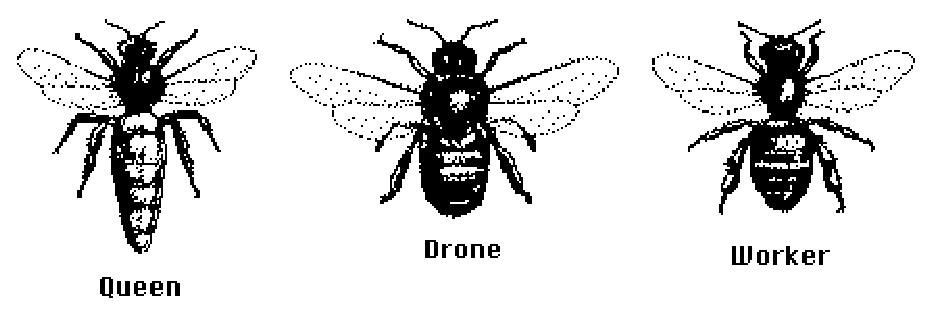
\includegraphics[height=3cm, angle=0]{threebees.eps}}
}

\author{Gerard Torrent Gironella}

\maketitle

\thispagestyle{empty}

\newpage

\vspace*{7in}

\noindent Copyright $\copyright$ 2004-2005 Gerard Torrent Gironella.  All rights reserved.\\

\noindent The image found in cover have been taken from Mark L. Winston. 1987. 
\emph{The Biology of the Honey Bee} (ISBN: 0-671-07109-2). Harvard University 
Press. Cambridge, MA. These redrawn figures appear here without permission of 
Harvard University Press [Ref: 973029].\\

\noindent This file is part of the CreditCruncher software package.  For
license information, see the LICENSE file in the top level directory
of the CreditCruncher source distribution.

\tableofcontents
%\listoftables


%***************************************************************************
%
% CreditCruncher - A portfolio credit risk valorator
% Copyright (C) 2004 Gerard Torrent
%
% This program is free software; you can redistribute it and/or
% modify it under the terms of the GNU General Public License
% as published by the Free Software Foundation; either version 2
% of the License.
%
% This program is distributed in the hope that it will be useful,
% but WITHOUT ANY WARRANTY; without even the implied warranty of
% MERCHANTABILITY or FITNESS FOR A PARTICULAR PURPOSE.  See the
% GNU General Public License for more details.
%
% You should have received a copy of the GNU General Public License
% along with this program; if not, write to the Free Software
% Foundation, Inc., 59 Temple Place - Suite 330, Boston, MA 02111-1307, USA.
%
%
% introduction.tex - TeX documentation file
% --------------------------------------------------------------------------
%
% 2004/12/04 - Gerard Torrent [gerard@fobos.generacio.com]
%   . initial release
%
%***************************************************************************

\chapter{Introduction to CreditCruncher}
\label{sec:introduction}

\section{About CreditCruncher}

CreditCruncher valora el riesgo de impago de una cartera de cr\'editos usando la 
t\'ecnica de simulaci\'on Monte Carlo. Es una implementaci\'on libre de la metodologia
CreditMetrics\footnote{http://www.riskmetrics.com/}. 

Se dispone de una cartera de N clientes donde cada cliente tiene contratado uno o 
varios productos con riesgo de crédito. Cada cliente tiene asignado un rating de 
calidad crediticia y existe una matriz de transición que permite determinar la 
probabilidad de fallido a un horizonte de tiempo fijado. Los clientes pertenecen 
a diversos sectores de los que disponemos de una matriz de correlación que 
indica el grado de dependencia intersectorial en caso de fallido. A partir de 
la matriz de correlación intersectorial se construye la matriz de correlación 
entre clientes. Finalmente se genera un conjunto de N variables aleatorias 
uniformes correlacionadas según esta matriz (cópula). Se usa la matriz de 
transición para determinar la evolución del rating inicial de cada cliente y se 
evalua el valor de sus productos. Si se repite este proceso un número elevado de 
veces disponemos de un conjunto de valores posibles de la cartera que permiten 
determinar la distribución del valor de la cartera y calcular el VAR (Value At Risk). 
Para mas información consúltese el manual de CreditCruncher donde se describe 
con detalle todos los pasos realizados.


\chapter{Formulaci\'on del problema}
\label{sec:formulation}

\section{Hipotesis}

\paragraph{La \'unica fuente de riesgo es el riesgo de impago.}
No se contemplan los riesgos de variación de tipos de interés, etc.

\paragraph{El tiempo est\'a repartido uniformemente.}
blablabla.

\paragraph{Un fallido no se recupera.}
blablabla.

\paragraph{Las probabilidades de fallido no dependen del tiempo.}
blablabla.

\paragraph{El rating y la recuperación de un cliente no depende de otro cliente.}
blablabla.


%===========================================================================

\section{La matriz de transición}

\subsection{Definici\'on.} La matriz de transición nos proporciona la probabilidad 
que un cliente con rating inicial $r_i$ pase a tener, al cabo de un tiempo $T$, 
rating $r_j$. La denotamos de la forma siguiente:

\begin{displaymath}
M_T = \left(
\begin{array}{ccc}
m_{1,1} & \dots  & m_{1,n} \cr
\vdots & \ddots & \vdots \cr
m_{n,1} & \dots  & m_{n,n} 
\end{array}
\right)
\end{displaymath}

\noindent donde cada elemento de la matrix, $m_{i,j}$ corresponde a la 
probabilidad de que un cliente con rating $r_i$ pase a tener, al cabo de $T$ 
tiempo, rating $r_j$.

\subsection{Ejemplo.} Matriz de transición anual ($T=1$ año) extraida del 
documento \emph{CreditMetrics. Technical Document}. Las probabilidades están
expresadas en tanto por ciento.
\\
\begin{center}
\begin{tabular}[]{l|rrrrrrrr}
        &      AAA &       AA &        A &      BBB &       BB &        B &      CCC &  Default \cr
\hline
AAA     &  $90.81$ &   $8.33$ &   $0.68$ &   $0.06$ &   $0.12$ &   $0.00$ &   $0.00$ &   $0.00$ \cr
 AA     &   $0.70$ &  $90.65$ &   $7.79$ &   $0.64$ &   $0.06$ &   $0.14$ &   $0.02$ &   $0.00$ \cr
  A     &   $0.09$ &   $2.27$ &  $91.05$ &   $5.52$ &   $0.74$ &   $0.26$ &   $0.01$ &   $0.06$ \cr
BBB     &   $0.02$ &   $0.33$ &   $5.95$ &  $86.93$ &   $5.30$ &   $1.17$ &   $0.12$ &   $0.18$ \cr
 BB     &   $0.03$ &   $0.14$ &   $0.67$ &   $7.73$ &  $80.53$ &   $8.84$ &   $1.00$ &   $1.06$ \cr
  B     &   $0.00$ &   $0.11$ &   $0.24$ &   $0.43$ &   $6.48$ &  $83.46$ &   $4.07$ &   $5.20$ \cr
CCC     &   $0.22$ &   $0.00$ &   $0.22$ &   $1.30$ &   $2.38$ &  $11.24$ &  $64.86$ &  $19.79$ \cr
Default &   $0.00$ &   $0.00$ &   $0.00$ &   $0.00$ &   $0.00$ &   $0.00$ &   $0.00$ & $100.00$
\end{tabular}
\end{center}
\noindent en particular, la probabilidad que un cliente con rating $AA$ pase a 
tener rating $B$ al cabo de un año es del $0.14\%$.

\subsection{Propiedades}

\paragraph{Propiedad 1.}
El valor de los elementos de la matriz de transici\'on se encuentran entre $0$ 
y $1$ debido a que son probabilidades.

\begin{displaymath}
0 \leq m_{i,j} \leq 1 \quad \forall i,j
\end{displaymath}

\paragraph{Propiedad 2.}
La suma de los elementos de cualquier fila de la matriz de transición suman $1$.
De esta forma se  está imponiendo que el conjunto de ratings finales solo puede 
ser el de los ratings contemplados en la matriz.

\begin{displaymath}
\sum_{j=1}^{n} m_{i,j} = 1 \quad \forall i
\end{displaymath}

\paragraph{Propiedad 3.}
Los elementos de la fila correspondiente al rating $default$, son todos $0$,
excepto el elemento de la columna que corresponde al rating $default$ que vale 
$1$. Esta condición indica que cuando se llega al estado de fallido no es 
posible salir de este estado.

\begin{displaymath}
\begin{array}{ll}
m_{default,j} = 0        & \quad \forall j \neq default \cr
m_{default,default} = 1
\end{array}
\end{displaymath}


\subsection{Cambio de periodo}

Deseamos obtener la matriz de transición para periodos distintos (múltiplos o 
fraccionarios) del periodo proporcionado, $T$. Esto nos permitirá determinar la 
probabilidad que un cliente con rating inicial $r_i$ tenga rating $r_j$ al cabo 
de $x \cdot T$ tiempo.

\paragraph{Ejemplo.} Calculemos la probabilidad de pasar de rating $AA$ a
rating $B$ en un plazo de dos años disponiendo de la matriz de transición anual.

\begin{displaymath}
\begin{array}{llll}
P(AA \to B;2) = & P(AA \to AAA;1)    & \cdot P(AAA \to B;1)      & + \cr
                & P(AA \to AA;1)      & \cdot P(AA \to B;1)      & + \cr
                & P(AA \to A;1)       & \cdot P(A \to B;1)       & + \cr
                & P(AA \to BBB;1)     & \cdot P(BBB \to B;1)     & + \cr
                & P(AA \to BB;1)      & \cdot P(BB \to B;1)      & + \cr
                & P(AA \to B;1)       & \cdot P(B \to B;1)       & + \cr
                & P(AA \to CCC;1)     & \cdot P(CCC \to B;1)     & + \cr
                & P(AA \to default;1) & \cdot P(default \to B;1) &
\end{array}
\end{displaymath}

\paragraph{Proposici\'on} Sean $M_{T_1}$ y $M_{T_2}$ las matrices de transici\'on
para los periodos $T_1$ y $T_2$. Entonces, la matriz de transici\'on para el
periodo $T_1+T_2$ es:
\begin{displaymath}
M_{T_1+T_2} = M_{T_1} \cdot M_{T_2}
\end{displaymath}

\paragraph{Corolario} Sean $M_{T}$ la matriz de transici\'on para el periodo 
$T$ y $k \in \mathrm{N}$. Entonces:
\begin{displaymath}
M_{k \cdot T} = M_{T}^k
\end{displaymath}
\begin{displaymath}
M_{\frac{T}{k}} = \sqrt[k]{M_{T}}
\end{displaymath}


%===========================================================================

\section{C\'alculo de la raiz de una matriz}

\paragraph{Definici\'on.}
Diremos que 2 matrices $A$ y $B$ de orden $n$ son semejantes si existe una 
matriz, $P$, de orden $n$ con $det(P) \neq 0$ tal que 
$B = P^{-1} \cdot A \cdot P$.


\paragraph{Proposici\'on.} Si dos matrices $A$ y $B$ son semejantes 
($B = P^{-1} \cdot A \cdot P$) entonces:
\begin{displaymath}
det(A) = det(B)
\end{displaymath}
\begin{displaymath}
B^n = P^{-1} \cdot A^{n} \cdot P
\end{displaymath}

\paragraph{Definici\'on.} 
Diremos que Una matriz $A$ de orden $n$ es diagonalizable si es semejante a una 
matriz diagonal $D$, o sea, $A = P^{-1} \cdot D \cdot P$ siendo $det(D) \neq 0$.

\paragraph{Proposici\'on.} 
Para que una matriz $A$ sea diagonalizable es necesario y suficiente que:
\begin{itemize}
\item Los valores propios de $A$ sean todos reales
\item Los $n$ vectores propios de $A$ sean independientes
\end{itemize}

\paragraph{Proposici\'on.}
Si una matriz $A$ es diagonalizable ($A = P^{-1} \cdot D \cdot P$) entonces: 
\begin{itemize}
\item $D$ es una matriz diagonal compuesta por los valores propios de la matriz $A$
\item $P$ es la matriz formada por los vectores propios de la matriz $A$
\end{itemize}

\paragraph{Resultado.}
Sea $A$ la raíz $n$-esima de una matriz diagonalizable $B$. Entonces:
\begin{displaymath}
A^n = B = P^{-1} \cdot D \cdot P 
\Longrightarrow  
A = \sqrt[n]{B} = P^{-1} \cdot \sqrt[n]{D} \cdot P
\end{displaymath} 


%===========================================================================

\section{Simulaci\'on de una variable aleatoria normal}

Para la generación de una realización, $z$, de una variable aleatoria normal  
$Z \sim N(\mu, \sigma)$ utilizamos el siguiente algoritmo:

\begin{displaymath}
z = \mu + \sigma\cdot \sqrt{-2 \cdot ln(u[0,1])} \cdot cos(2 \cdot \pi \cdot u[0,1])
\end{displaymath}

\noindent donde $u[0,1]$ son realizaciones de una variable aleatoria uniforme 
en el intervalo $[0,1]$.

%===========================================================================

\section{Copulas. Variables aleatorias correlacionadas}

\paragraph{Definici\'on.}
Una copula es la funci\'on de distribuci\'on de un vector aleatorio sobre 
$\Re^n$ donde las funciones de distribuci\'on marginales son $U[0,1]$. Se 
puede demostrar que esta definici\'on es equivalente a definir una copula
como una funci\'on $C:[0,1]^n \to [0,1]$ cumpliendo las siguientes propiedades:
\begin{itemize}
\item $C(x_1, \cdots, x_n)$ es creciente en cada componente $x_i$
\item $C(1, \cdots, 1, x_i, 1, \cdots, 1) = x_i \quad \forall i \in \{1, \cdots, n\}, x_i \in [0,1]$
\item $\forall (a_1, \cdots, a_n) \in [0,1]^n$ y $\forall (b_1, \cdots, b_n) \in [0,1]^n$ con
$a_i \leq b_i$ se cumple:
\begin{displaymath}
\sum_{i_1=1}^{2} \cdots \sum_{i_n=1}^{2} (-1)^{i_1+\cdots+x_n} C(x_{1i_1},\cdots,x_{ni_n}) \geq 0
\end{displaymath}
\end{itemize}
\noindent siendo $x_{j1}=a_j$ y $x_j2=b_j$ $\quad \forall j \in \{1, \cdots, n\}$









%***************************************************************************
%
% CreditCruncher - A portfolio credit risk valorator
% Copyright (C) 2004 Gerard Torrent
%
% This program is free software; you can redistribute it and/or
% modify it under the terms of the GNU General Public License
% as published by the Free Software Foundation; either version 2
% of the License.
%
% This program is distributed in the hope that it will be useful,
% but WITHOUT ANY WARRANTY; without even the implied warranty of
% MERCHANTABILITY or FITNESS FOR A PARTICULAR PURPOSE.  See the
% GNU General Public License for more details.
%
% You should have received a copy of the GNU General Public License
% along with this program; if not, write to the Free Software
% Foundation, Inc., 59 Temple Place - Suite 330, Boston, MA 02111-1307, USA.
%
%
% formulation.tex - TeX documentation file - $Rev$
% --------------------------------------------------------------------------
%
% 2005/01/22 - Gerard Torrent [gerard@fobos.generacio.com]
%   . initial release
%
% 2005/10/15 - Gerard Torrent [gerard@fobos.generacio.com]
%   . added Rev (aka LastChangedRevision) svn tag
%
%***************************************************************************

\chapter{Formulaci\'on}
\label{sec:formulation}

\begin{center}
\framebox{
\begin{minipage}[c]{12.5cm}
Dada una cartera de cr\'editos a empresas de tama\~no mediano, deseamos 
valorar el riesgo debido a los impagos al cabo de un                                                                                                                                         tiempo $T$.
\end{minipage}
}
\end{center}

A continuaci\'on se introduce los elementos y propiedades b\'asicas que 
constituyen el marco de trabajo.

%---------------------------------------------------------------------------

\section{Cartera de cr\'editos}

La estructura de la cartera de cr\'editos consiste en un conjunto de
clientes agrupados por sectores de actividad. Cada cliente tiene contratado 
un conjunto de productos de cr\'edito. Cada contrato puede estar 
cubierto por un n\'umero variable de garant\'ias o acuerdos.
Puede verse un esquema de la estructura en la figura \ref{portfolio}.

\begin{figure}[!hb]
\begin{center}
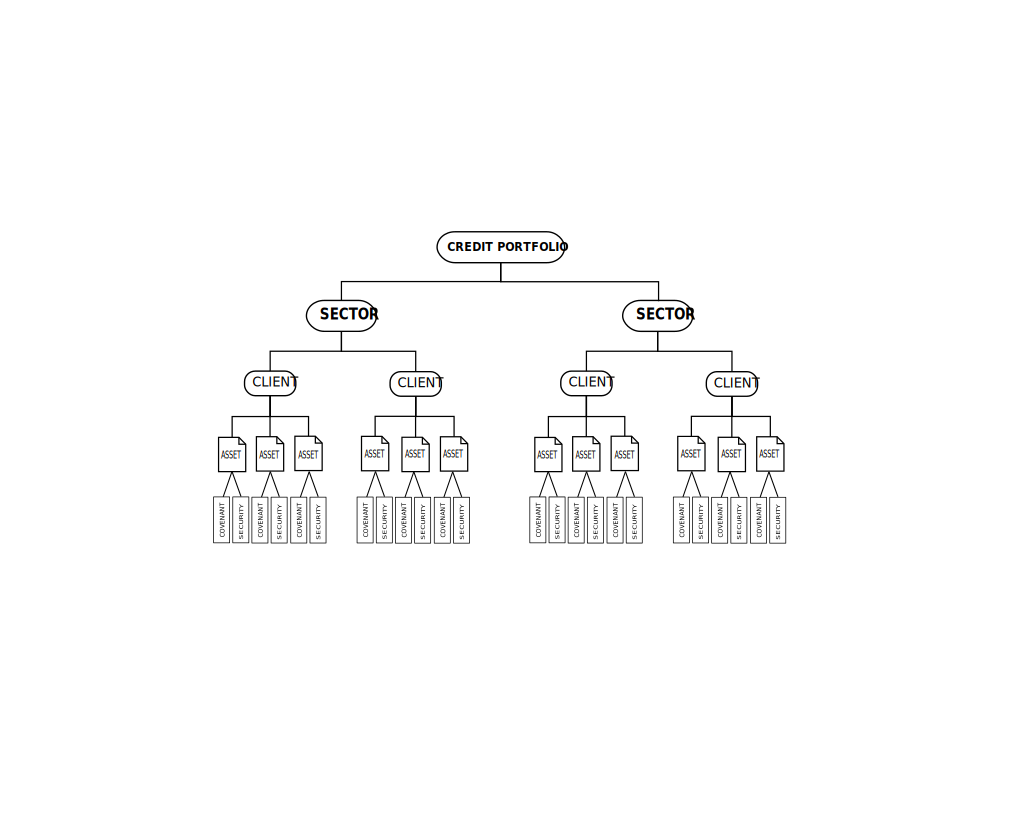
\includegraphics[width=6cm,angle=-90]{./images/portfolio.epsi}
\caption{Estructura de la cartera de cr\'editos}
\label{portfolio}
\end{center}
\end{figure}


\subsection{Ratings}

Un \emph{sistema de ratings}\index{Sistema de ratings} es una medida de calidad
crediticia usada para valorar creditores. A cada creditor se le asigna una nota
discreta (pe. AAA, AA, A, BBB, BB, B, CCC, Default) en funci\'on de su calidad
crediticia. Los \'unicos ratings contemplados en este documento 
son los que tienen una relaci\'on estad\'istica directa y cuantificable 
con la probabilidad de impago del creditor. Ejemplos de este tipo de ratings 
son los publicados por Moody's Investor Service\footnote{http://www.moodys.com} 
o Standard \& Poors\footnote{http://www.standardandpoors.com}. 
\newline
\newline
La metodolog\'ia para la generaci\'on de un sistema de ratings queda fuera del
\'ambito de este documento. CreditCruncher presupone que cada empresa de la 
cartera tiene un rating inicial asignado.
\newline
\newline
El rating de cada empresa puede variar a lo largo del tiempo (v\'ease figura
\ref{ratingevol}). La evoluci\'on temporal del rating de una empresa se
contempla a trav\'es de la matriz de transici\'on o la funci\'on de 
supervivencia (v\'ease la secci\'on \ref{sec:mtransition}).
\begin{figure}[!hb]
\begin{center}
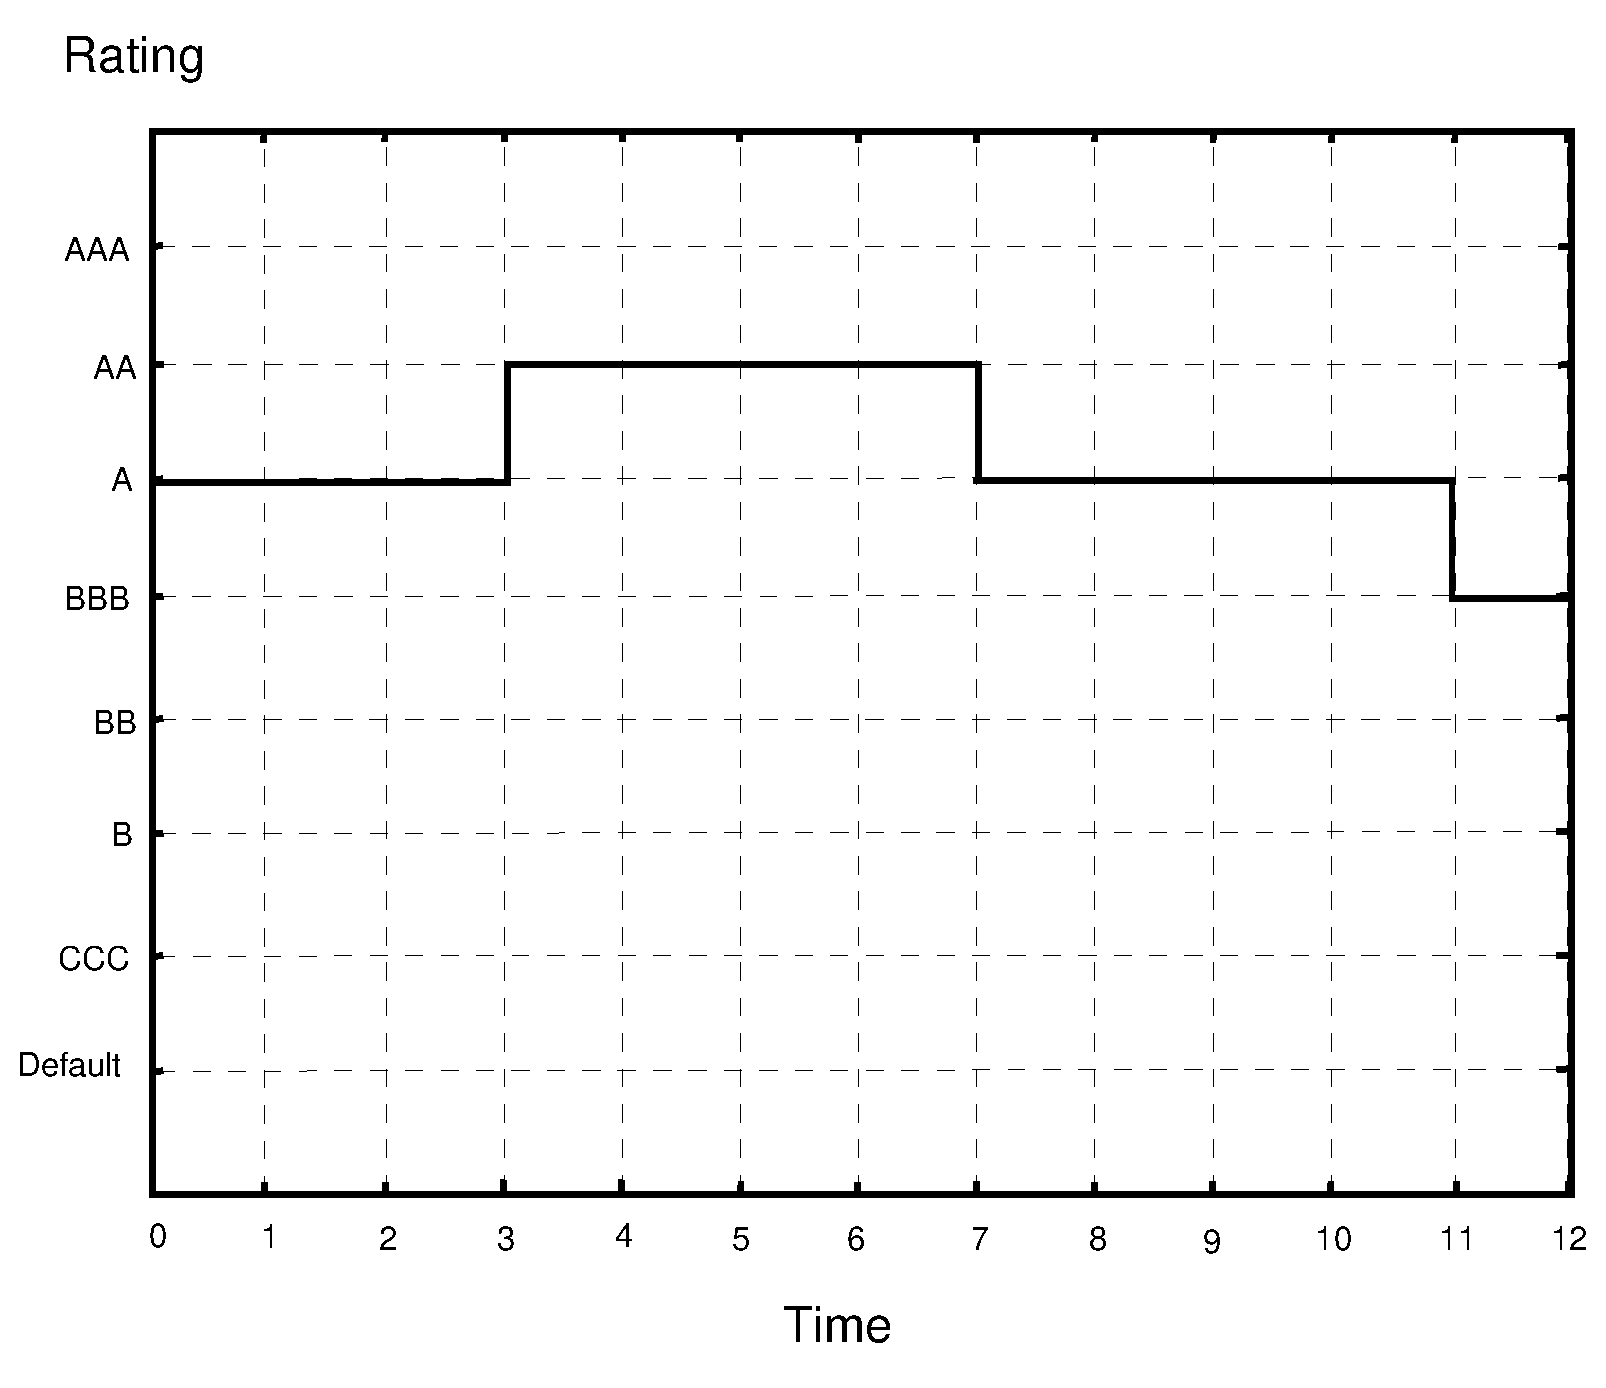
\includegraphics[height=6cm, angle=0]{./images/ratingevol.eps}
\caption{Evoluci\'on del rating a lo largo del tiempo}
\label{ratingevol}
\end{center}
\end{figure}

\paragraph{Notaci\'on.} $rating(i,t) =$ rating del cliente $i$ en el tiempo $t$.

\paragraph{Notaci\'on.} $P(r_i \to r_j;t_0;t_1) =$ probabilidad de pasar de un 
rating inicial $r_i$ en tiempo $t_0$ a un rating $r_j$ en tiempo $t_1$.


\subsection{Sectores}

La correlaci\'on de fallidos entre clientes es uno de los conceptos que
a\~naden complejidad de la valoraci\'on del riesgo de cr\'edito. No es lo
mismo tener una cartera de cr\'editos donde los clientes hacen fallido 
de forma independiente que una cartera donde los fallidos se encuentran 
correlacionados. En el primer caso, al cabo de un a\~no tendremos un 
conjunto limitado de fallidos. En el segundo caso, al cabo de un a\~no la 
mayor\'ia de clientes habr\'an hecho fallido o casi ning\'un cliente habr\'a
hecho fallido.

\begin{figure}[!hb]
\begin{center}
\includegraphics[width=6cm,angle=-90]{./images/sectorcorrel.ps}
\caption{Impacto de la correlaci\'on intrasectorial}
\label{sectorcorrel}
\end{center}
\end{figure}

Al no poder asignar una correlaci\'on de fallido cliente a cliente, se recurre
a la agrupaci\'on de estos en \emph{sectores}\index{Sectores}. Se considera que
la cartera de cr\'editos dispone de un conjunto de sectores donde los componentes
de cada sector muestran una evoluci\'on crediticia similar. O sea, que la mejora
o empeoramiento de la calidad crediticia (rating) afecta de forma com\'un a los
componentes del sector. En general se identifican estos sectores con los 
sectores industriales. 
\newline
\newline
Se considera que cada cliente pertenece a un \'unico sector y permanece en 
el a lo largo del tiempo. La relaci\'on entre sectores se contempla a trav\'es 
de la tabla de correlaciones sectoriales (v\'ease la secci\'on \ref{sec:mcorrel}).

\paragraph{Notaci\'on.} $sector(i) =$ sector al que pertenece el cliente $i$.

\subsection{Activos}

Cada cliente tiene contratado un conjunto de activos con riesgo de cr\'edito.
Caracterizamos un activo por los siguientes elementos (importes positivos
significan que el cliente paga, importes negativos significan que el cliente 
cobra):

\paragraph{Cashflow.} \index{Cashflow} Entregas y devoluciones de dinero a lo largo
del tiempo. Incluye las posibles amortizaciones, primas, cupones, comisiones, costes,
etc. Usaremos el cashflow para calcular el valor, o precio, de un activo en el
instante $t$.

\paragraph{Recovery.} \index{Recovery} Importe correspondiente a la
liquidaci\'on de deudas mutuas en caso de fallido. Incluye la posible recuperaci\'on,
pago de obligaciones contra\'idas (pe. en el caso de avales), etc. Puede equipararse
a $EAD \times (1-LGD)$ donde $EAD$ es Exposure At Default \index{EAD} (importe) y
$LGD$ es Loss Given Default \index{LGD} (porcentaje).

\paragraph{Ejemplo.}
Caracterizamos un bono (bond) de $100$ \euro~ de valor nominal, con fecha emisi\'on
31/12/2006, tipo de inter\'es anual del $4\%$, pago anual de cupones y amortizaci\'on
al cabo de $5$ a\~nos. En caso de fallido se estima que se recupera un $80\%$ del
importe pendiente de abonar.\newline

\begin{center}
\begin{tabular}{c|r|r}
\textbf{Date} & \textbf{Cashflow} & \textbf{Recovery} \\
\hline
31/12/2006 &  -100.00 &    0.00 \\
31/12/2007 &     4.00 &   96.00 \\
31/12/2008 &     4.00 &   92.00 \\
31/12/2009 &     4.00 &   89.60 \\
31/12/2010 &     4.00 &   86.40 \\
31/12/2011 &   104.00 &   83.20
\end{tabular}
\end{center}

\paragraph{Ejemplo.}
Caracterizamos un pr\'estamo hipotecario (mortgage) de $100$ \euro, con fecha
de contrataci\'on 15/01/2006, tipo de inter\'es anual del $6.5\%$ y cuota
(instalment) mensual y un plazo de $25$ a\~nos. La vivienda hipotecada est\'a
valorada en $80$ \euro. Determinamos la cuota mensual usando la siguiente
f\'ormula (canon vencido o m\'etodo franc\'es):
\begin{displaymath}
I =
\frac{A \cdot r \cdot (1+r)^t}{(1+r)^t - 1} =
\frac{100 \cdot (6.5\%/12) \cdot (1+6.5\%/12)^{25\cdot12}}{(1+6.5\%/12)^{25\cdot12} - 1} =
0.67521
\end{displaymath}

\begin{center}
\begin{tabular}{c|r|r}
\textbf{Date} & \textbf{Cashflow} & \textbf{Recovery} \\
\hline
15/01/2006 &  -100.00 &    0.00 \\
15/02/2006 &     0.68 &   80.00 \\
15/03/2006 &     0.68 &   80.00 \\
15/04/2006 &     0.68 &   80.00 \\
\dots      &    \dots &   \dots \\
15/11/2030 &     0.68 &   80.00 \\
15/12/2030 &     0.68 &   80.00 \\
15/01/2031 &     0.68 &   80.00
\end{tabular}
\end{center}

\paragraph{Ejemplo.}
Caracterizamos un aval (endorsement) por un importe avalado de $100$ \euro~
con fecha de contrataci\'on 15/01/2006, durante un periodo de $2$ a\~nos y
una cuota semestral anticipada de $4.5$ \euro.

\begin{center}
\begin{tabular}{c|r|r}
\textbf{Date} & \textbf{Cashflow} & \textbf{Recovery} \\
\hline
15/01/2006 &     4.50 &    0.00 \\
15/07/2006 &     4.50 & -100.00 \\
15/01/2007 &     4.50 & -100.00 \\
15/07/2007 &     4.50 & -100.00 \\
15/01/2008 &     0.00 & -100.00
\end{tabular}
\end{center}


%---------------------------------------------------------------------------

\section{Tipos de inter\'es}
\label{sec:interests}

\paragraph{Definici\'on.}
Sea $C_{t_0}$ el importe inicial de una operaci\'on y $C_{t_1}$ el importe final. 
Definimos el \emph{tipo de inter\'es efectivo}\index{Tipo de inter\'es efectivo}, $r$,
como:
\begin{equation}
C_{t_1} = C_{t_0} \cdot (1+r)
\end{equation}

\begin{equation}
\label{tipus_efectiu}
r = \frac{C_{t_1}-C_{t_0}}{C_{t_0}}
\end{equation}

\paragraph{Definici\'on.}
El \emph{tipo de inter\'es simple}\index{Tipo de inter\'es simple}, $r_s$, es un tipo
de inter\'es donde para cada periodo de tiempo se incrementa el importe inicial, $C_{t_0}$
por un factor de $r_s$.
\begin{equation}
C_{t_1} = C_{t_0} \cdot (1+ r_s \cdot (t_1-t_0))
\end{equation}

\begin{equation}
\label{interes_simple_1}
r_s = \frac{r}{t_1 - t_0}
\end{equation}

\paragraph{Definici\'on.}
El \emph{tipo de inter\'es compuesto}\index{Tipo de inter\'es compuesto}, $r_c$, es un tipo
de inter\'es donde en cada periodo de tiempo se incrementa por un factor de $r_c$ el importe
acumulado del periodo anterior.
\begin{equation}
C_{t_1} = C_{t_0} \cdot (1+ r_c)^{(t_1-t_0)}
\end{equation}

\begin{equation}
\label{interes_compuesto_1}
r_c = (1 + r) ^ \frac{1}{t_1-t_0} - 1
\end{equation}

\paragraph{Definici\'on.}
El \emph{tipo de inter\'es continuo}\index{Tipo de inter\'es continuo}, $r_e$, es el caso
l\'\i mite del inter\'es compuesto.
\begin{equation}
C_{t_1} = C_{t_0} \cdot e^{r_e \cdot (t_1-t_0)}
\end{equation}

\begin{equation}
\label{interes_continuo_1}
r_e = \ln(1 + r_c)
\end{equation}

La f\'ormula exponencial, no el coeficiente, se obtiene considerando el
l\'\i mite del tipo de inter\'es compuesto.
\begin{equation}
\label{interes_continuo_2}
\begin{array}{c}
\lim_{t_1 \rightarrow t_0} 1+r_c = 
\lim_{t_1 \rightarrow t_0} (1 + r)^{\frac{1}{t_1 - t_0}} = \cr
\lim_{t_1 \rightarrow t_0} (1 + r_s \cdot (t_1-t_0)) ^ {\frac{1}{t_1 - t_0}} =
\lim_{n \rightarrow \infty} (1 + \frac{r_s}{n}) ^ {n} = 
e^{r_s}
\end{array}
\end{equation}

\paragraph{Ejemplo.}
Consideremos una operaci\'on que supone una inversi\'on inicial de 100 MM. y que 
al cabo de 5 a\~{n}os proporciona unos ingresos de 120 MM. 
\newline
\newline
Calculemos los diferentes tipos de inter\'es:
\begin{displaymath}
\begin{array}{l}
r = \frac{120-100}{100} = 20 \% \cr
r_s= \frac{r}{5} = \frac{20 \%}{5} = 4 \% \cr
r_c= (1+r) ^ {1/5} - 1 = 1.2^{0.2} - 1 = 1.0371 - 1 = 3.71 \% \cr
r_e= \ln(1 + r_c) = \ln(1.0371) = 3.65 \%
\end{array}
\end{displaymath}
\newline
\newline
Recuperemos el importe final de la operaci\'on a partir del importe inicial, 
el intervalo de tiempo y el tipo de inter\'es:
\begin{displaymath}
\begin{array}{lcl}
\textrm{tipo efectivo}       & \rightarrow & C_{t_1} = 100 \cdot (1 + 20\%) = 120 \cr
\textrm{inter\'es simple}    & \rightarrow & C_{t_1} = 100 \cdot (1 + 4\% \cdot 5) = 120 \cr
\textrm{inter\'es compuesto} & \rightarrow & C_{t_1} = 100 \cdot (1 + 3.71\%)^5 = 120 \cr
\textrm{inter\'es continuo}  & \rightarrow & C_{t_1} = 100 \cdot e^{3.65 \% \cdot 5} = 120
\end{array}
\end{displaymath}

\subsection{Funci\'on de transporte}

\paragraph{Definici\'on.} Fijado un tipo de inter\'es, $r$, y un intervalo de
tiempo, $\Delta t = t_k-t_0$, \emph{la funci\'on de transporte}\index{Funci\'on de transporte},
$\Upsilon$, proporciona el factor que debe aplicarse a un importe en $t_0$ para obtener el
importe equivalente en $t_k$.
\newline
\newline
Caso $C_0 \longrightarrow C_k \quad t_0 < t_k$:
\begin{displaymath}
\begin{array}{lcl}
\textrm{inter\'es simple}    & \rightarrow & C_0 \cdot \Upsilon(t_0,t_k, r) = C_0 \cdot (1+r\cdot(t_k-t_0)) = C_k \cr
\textrm{inter\'es compuesto} & \rightarrow & C_0 \cdot \Upsilon(t_0,t_k, r) = C_0 \cdot (1+r)^{(t_k-t_0)} = C_k \cr
\textrm{inter\'es continuo}  & \rightarrow & C_0 \cdot \Upsilon(t_0,t_k, r) = C_0 \cdot e^{r\cdot(t_k-t_0)} = C_k 
\end{array}
\end{displaymath}
Caso $C_k \longleftarrow C_0 \quad t_k < t_0$:
\begin{displaymath}
\begin{array}{lcl}
\textrm{inter\'es simple}    & \rightarrow & C_0 \cdot \Upsilon(t_0,t_k, r) = C_0 \cdot (1+r\cdot(t_0-t_k))^{-1} = C_k \cr
\textrm{inter\'es compuesto} & \rightarrow & C_0 \cdot \Upsilon(t_0,t_k, r) = C_0 \cdot (1+r)^{-(t_0-t_k)} = C_k \cr
\textrm{inter\'es continuo}  & \rightarrow & C_0 \cdot \Upsilon(t_0,t_k, r) = C_0 \cdot e^{-r\cdot(t_0-t_k)} = C_k
\end{array}
\end{displaymath}

\paragraph{Notaci\'on.} En este documento se considera que el tipo de inter\'es
aplicado es el tipo de inter\'es compuesto. En este caso, la funci\'on de transporte
tiene una expresi\'on \'unica, sea cual sea el sentido en el que se aplica:
\begin{equation}
\label{funcion_transporte_1}
\Upsilon(t_0,t_k, r) = (1+r)^{(t_k-t_0)}
\end{equation}


\subsection{Curva spot o cup\'on cero}

\paragraph{Definici\'on.} La \emph{curva spot}\index{Curva spot} o
\emph{curva cup\'on cero}\index{Curva cup\'on cero} es la funci\'on
$S$ que indica el tipo de inter\'es a aplicar en la funci\'on de transporte
desde el tiempo $t_0$.

En el mercado existen productos simples a distintos plazos para los cuales se 
puede calcular el tipo de inter\'es que proporcionan. Estos tipos de inter\'es
solamente se pueden usar en la funci\'on de transporte cuando uno de los
tiempos sea $t_0$ y el otro sea superior a $t_0$.

\begin{figure}[!hb]
\begin{center}
\includegraphics[height=10cm, angle=-90]{./images/spot.ps}
\caption{Curva Spot}
\label{spot}
\end{center}
\end{figure}

\paragraph{Proposici\'on.} Dada una curva spot $S_{t_0}$ en $t_0$, podemos calcular
el coeficiente de transporte entre $t_i$ y $t_j$ para todo $t_i, t_j \ge t_0$:
\begin{equation}
\Upsilon_S(t_i,t_j) =
\Upsilon(t_i,t_0, S_{t_0}(t_i)) \cdot \Upsilon(t_0,t_j, S_{t_0}(t_j))
\end{equation}


%---------------------------------------------------------------------------

\section{Matriz de transici\'on}
\label{sec:mtransition}

\paragraph{Definici\'on.} La \emph{matriz de transici\'on}\index{Matriz de transici\'on}
en el periodo $T$ es una matriz cuadrada que proporciona la probabilidad que un cliente
con rating inicial $r_i$ pase a tener, al cabo de un tiempo $T$, rating $r_j$.
La denotamos de la forma siguiente:
\begin{displaymath}
M_T = \left(
\begin{array}{ccc}
m_{1,1} & \dots  & m_{1,n} \cr
\vdots & \ddots & \vdots \cr
m_{n,1} & \dots  & m_{n,n} 
\end{array}
\right)
\qquad
m_{i,j} = P(r_i \to r_j;0;T)
\end{displaymath}

donde $n$ es el n\'umero de ratings y $m_{i,j}$ corresponde a la probabilidad de que un
cliente con rating $r_i$ pase a tener, al cabo de $T$ tiempo, rating $r_j$.

\paragraph{Ejemplo.} Matriz de transici\'on anual ($T=1$ a\~no).
Las probabilidades est\'an expresadas en tanto por ciento.
\\
\begin{center}
\begin{tabular}[]{l|rrrrrrrr}
        &      AAA &       AA &        A &      BBB &       BB &        B &      CCC &  Default \cr
\hline
AAA     &  $90.81$ &   $8.33$ &   $0.68$ &   $0.06$ &   $0.12$ &   $0.00$ &   $0.00$ &   $0.00$ \cr
 AA     &   $0.70$ &  $90.65$ &   $7.79$ &   $0.64$ &   $0.06$ &   $0.14$ &   $0.02$ &   $0.00$ \cr
  A     &   $0.09$ &   $2.27$ &  $91.05$ &   $5.52$ &   $0.74$ &   $0.26$ &   $0.01$ &   $0.06$ \cr
BBB     &   $0.02$ &   $0.33$ &   $5.95$ &  $86.93$ &   $5.30$ &   $1.17$ &   $0.12$ &   $0.18$ \cr
 BB     &   $0.03$ &   $0.14$ &   $0.67$ &   $7.73$ &  $80.53$ &   $8.84$ &   $1.00$ &   $1.06$ \cr
  B     &   $0.00$ &   $0.11$ &   $0.24$ &   $0.43$ &   $6.48$ &  $83.46$ &   $4.07$ &   $5.21$ \cr
CCC     &   $0.22$ &   $0.00$ &   $0.22$ &   $1.30$ &   $2.38$ &  $11.24$ &  $64.86$ &  $19.78$ \cr
Default &   $0.00$ &   $0.00$ &   $0.00$ &   $0.00$ &   $0.00$ &   $0.00$ &   $0.00$ & $100.00$
\end{tabular}
\end{center}
En particular, la probabilidad que un cliente con rating $AA$ pase a tener 
rating $B$ al cabo de $1$ a\~no es del $0.14\%$.

\subsection{Propiedades}
\label{sec:mtransition:properties}

\paragraph{Propiedad 1.}
El valor de los elementos de la matriz de transici\'on se encuentra entre $0$ 
y $1$ debido a que los elementos de la matriz son probabilidades.

\begin{equation}
0 \leq m_{i,j} \leq 1 \quad \forall i,j
\end{equation}

\paragraph{Propiedad 2.}
La suma de los elementos de cualquier fila de la matriz de transici\'on vale $1$.
De esta forma se  est\'a imponiendo que el conjunto de ratings finales solo puede 
ser el de los ratings contemplados en la matriz.

\begin{equation}
\sum_{j=1}^{n} m_{i,j} = 1 \quad \forall i
\end{equation}

\paragraph{Propiedad 3.}
Los elementos de la fila correspondiente al rating $Default$ ($r_n$), son todos 
$0$, excepto el elemento de la columna que corresponde al rating $Default$, 
$m_{n,n}$, que vale $1$. Esta condici\'on indica que cuando se llega al estado 
de fallido no es posible salir de este estado.

\begin{equation}
\begin{array}{ll}
m_{n,j} = 0        & \quad \forall j \neq n \cr
m_{n,n} = 1
\end{array}
\end{equation}

\paragraph{Propiedad 4.}
Sea cual sea el rating inicial, existe la posibilidad que realice fallido.

\begin{equation}
\forall i \quad \exists j \quad \textrm{tq.} \quad m_{i,j} > 0 \quad \textrm{and} \quad  m_{j,n} > 0
\end{equation}

\paragraph{Propiedad 5.}
La matriz de transici\'on es diagonalizable. O sea, todos los valores propios son
reales e independientes.

\begin{equation}
M_{T} \quad \textrm{is diagonalizable}
\end{equation}

Esta propiedad es una condici\'on t\'ecnica para garantizar la existencia de las
raices de la matriz de transici\'on.


\subsection{Cambio de periodo}
\label{mtrans:perchange}

Deseamos obtener la matriz de transici\'on para periodos distintos (m\'ultiplos o 
fraccionarios) del periodo proporcionado, $T$. Esto nos permitir\'a determinar la 
probabilidad que un cliente con rating inicial $r_i$ tenga rating $r_j$ al cabo 
de $k \cdot T$ tiempo o al cabo de $T/k$ tiempo.

\paragraph{Ejemplo.} Calculemos la probabilidad de pasar de rating $AA$ a
rating $B$ en un plazo de dos a\~nos disponiendo de la matriz de transici\'on anual.

\begin{displaymath}
\begin{array}{llll}
P(AA \to B;0;2) = & P(AA \to AAA;0;1)     & \cdot P(AAA \to B;1;2)     & + \cr
                  & P(AA \to AA;0;1)      & \cdot P(AA \to B;1;2)      & + \cr
                  & P(AA \to A;0;1)       & \cdot P(A \to B;1;2)       & + \cr
                  & P(AA \to BBB;0;1)     & \cdot P(BBB \to B;1;2)     & + \cr
                  & P(AA \to BB;0;1)      & \cdot P(BB \to B;1;2)      & + \cr
                  & P(AA \to B;0;1)       & \cdot P(B \to B;1;2)       & + \cr
                  & P(AA \to CCC;0;1)     & \cdot P(CCC \to B;1;2)     & + \cr
                  & P(AA \to Default;0;1) & \cdot P(Default \to B;1;2) &
\end{array}
\end{displaymath}

Notamos que se trata del producto de la fila correspondiente al rating $AA$ 
(rating de salida) por la columna correspondiente al rating $B$ (rating de 
llegada).

\paragraph{Proposici\'on.} Sean $M_{T_1}$ y $M_{T_2}$ las matrices de transici\'on
para los periodos $T_1$ y $T_2$. Entonces, la matriz de transici\'on para el
periodo $T_1+T_2$ es:
\begin{equation}
M_{T_1+T_2} = M_{T_1} \cdot M_{T_2}
\end{equation}

\paragraph{Corolario.} Sean $M_{T}$ la matriz de transici\'on para el periodo 
$T$ y $k \in \mathrm{N}$. Entonces\footnote{v\'ease el ap\'endice \ref{apendix:sqrtmat} 
para ver como se calcula la ra\'iz de una matriz}:
\begin{equation}
M_{k \cdot T} = M_{T}^k
\end{equation}
\begin{equation}
M_{\frac{T}{k}} = \sqrt[k]{M_{T}}
\end{equation}


\subsection{Funci\'on de supervivencia}
\label{mtrans:survival}

\paragraph{Definici\'on.} La \emph{Tasa de Morosidad Anticipada Acumulada}
o \emph{Cumulated Forward Default Rate}\index{Cumulated Forward Default Rate} (CFDR)
del rating $r_i$ en el tiempo $t$ es la probabilidad que una empresa con rating inicial
$r_i$ haga fallido en el intervalo de tiempo $(0,t)$.

\begin{equation}
CFDR(r_i,t)=P(r_i \to Default;0;t)
\end{equation}

\begin{figure}[!hb]
\begin{center}
\includegraphics[height=10cm, angle=-90]{./images/tmaa.ps}
\caption{Tasa de Morosidad Anticipada Acumulada (CFDR)}
\label{cfdr}
\end{center}
\end{figure}

\paragraph{Definici\'on.} La \emph{Supervivencia}\index{Supervivencia} en el
tiempo $t$ del rating $r_i$ es la probabilidad que una empresa con rating inicial
$r_i$ no haya hecho fallido en el intervalo de tiempo $(0,t)$.

\begin{figure}[!hb]
\begin{center}
\includegraphics[height=10cm, angle=-90]{./images/survival.ps}
\caption{Funci\'on de Supervivencia}
\label{survival}
\end{center}
\end{figure}

\paragraph{Proposici\'on.} La Tasa de Morosidad Anticipada Acumulada se 
puede expresar en funci\'on de la matriz de transici\'on a trav\'es de la
relaci\'on siguiente:
\begin{equation}
CFDR(r_i,k \cdot T) = (M_{k \cdot T})_{i,n} = (M_{T}^{k})_{i,n}
\label{eq:cdfr1}
\end{equation}
donde $n$ es el \'indice del rating Default y $T$ es el periodo de la matriz
de transici\'on.

\paragraph{Proposici\'on.} La Supervivencia puede expresarse en funci\'on de
la Tasa de Morosidad Anticipada Acumulada a trav\'es de la relaci\'on siguiente:
\begin{equation}
Survival(r_i, t) =  1 - CFDR(r_i, t)
\label{eq:survival1}
\end{equation}

\paragraph{Proposici\'on.} Si la matriz de transici\'on es v\'alida, cualquier 
rating inicial acaba haciendo fallido casi seguramente.
\begin{equation}
lim_{t \to \infty} CFDR(r_i, t) =  1 \quad \forall i
\end{equation}

\paragraph{Proposici\'on.} Fijado un rating, $r_i$, la funci\'on de 
supervivencia es mon\'otona decreciente. Si el rating es $Default$,
el valor de la funci\'on de supervivencia es siempre $0$.
\begin{equation}
\label{prop:survival1}
Survival(r_i, t_j) \ge Survival(r_i, t_k) \quad \forall t_j < t_k
\end{equation}
\begin{equation}
\label{prop:survival2}
Survival(Default, t) = 0 \quad \forall t
\end{equation}

\paragraph{Ejemplo.} En las figuras \ref{cfdr} y \ref{survival} se puede observar
la Tasa de Morosidad Anticipada Acumulada y la Funci\'on de Supervivencia de la matriz
de transici\'on usada en este documento.

%---------------------------------------------------------------------------

\section{Matriz de correlaci\'on}
\label{sec:mcorrel}

\paragraph{Definici\'on.} La \emph{tabla de correlaciones sectoriales}
\index{Tabla de correlaciones sectoriales} proporciona la correlaci\'on de los
fallidos entre los sectores. La denotamos de la forma siguiente:

\begin{center}
\begin{tabular}[]{c|ccc}
             & $Sector_1$     & $\dots$  & $Sector_{m}$   \cr
\hline
$Sector_1$   & $\gamma_{1,1}$ & $\dots$  & $\gamma_{1,m}$ \cr
$\vdots$     & $\vdots$       & $\ddots$ & $\vdots$       \cr
$Sector_{m}$ & $\gamma_{1,m}$ & $\dots$  & $\gamma_{m,m}$ \cr
\end{tabular}
\end{center}

donde $m$ es el n\'umero de sectores, $\gamma_{i,j} = Corr(Sector_i, Sector_j)$
es la correlaci\'on entre los fallidos de los sectores $i$ y $j$ y $\gamma_{i,i}$ es
la correlaci\'on del fallido entre las empresas del sector $i$.No se trata de una verdadera
matriz de correlaci\'on debido a que la diagonal puede ser distinta de $1$.

\paragraph{Definici\'on.} La \emph{matriz de correlaci\'on entre clientes}
\index{Matriz de correlaci\'on entre clientes} proporciona la correlaci\'on de los
fallidos entre clientes. La construimos a partir de la tabla de correlaciones sectoriales
de la forma siguiente:
\begin{displaymath}
\Theta = \left(
\begin{array}{ccccc}
1              & \theta_{1,2}   & \dots      & \theta_{1,p-1} & \theta_{1,p}   \cr
\theta_{1,2}   & 1              & \dots      & \theta_{2,p-1} & \theta_{2,p}   \cr
\vdots         & \vdots         & \ddots     & \vdots         & \vdots         \cr
\theta_{1,p-1} & \theta_{2,p-1} & \dots      & 1              & \theta_{p-1,p} \cr
\theta_{1,p}   & \theta_{2,p}   & \dots      & \theta_{p-1,p} & 1
\end{array}
\right)
\end{displaymath}
donde $p$ es el n\'umero de clientes y $\theta_{i,j}$ es la correlaci\'on sectorial
entre el sector del cliente $i$ y el sector del cliente $j$. Por construcci\'on, la
matriz de correlaci\'on entre clientes es sim\'etrica debido a que la correlaci\'on
entre del sector del cliente $i$ con el sector del cliente $j$ es la misma que la
correlaci\'on del sector del cliente $j$ con el sector del cliente $i$.

\paragraph{Observaci\'on.} Los clientes se acostumbran a ordenar por sectores. En este
caso la matriz de correlaci\'on entre clientes queda de la forma siguiente:
\begin{displaymath}
\begin{array}{c}
\Theta = \\
\left(
\begin{array}{ccccccccccc}
1                & \dots    & \gamma_{p_1,p_1}  &          & \gamma_{1,p_i}   & \dots   & \gamma_{1,p_i}    &         & \gamma_{1,p_m}   & \dots      & \gamma_{1,p_m}   \cr
\vdots           & \ddots   & \vdots            &          & \vdots           &         & \vdots            &         & \vdots           &            & \vdots           \cr
\gamma_{p_1,p_1} & \dots    & 1                 &          & \gamma_{1,p_i}   & \dots   & \gamma_{1,p_i}    &         & \gamma_{1,p_m}   & \dots      & \gamma_{1,p_m}   \cr

                 &          &                   & \ddots   &                  &         &                   &         &                  &            &                  \cr

\gamma_{1,p_i}   & \dots    & \gamma_{1,p_i}    &          & 1                & \dots   & \gamma_{p_i,p_i}  &         & \gamma_{p_i,p_m} & \dots      & \gamma_{p_i,p_m} \cr
\vdots           & \ddots   & \vdots            &          & \vdots           & \ddots  & \vdots            &         & \vdots           &            & \vdots           \cr
\gamma_{1,p_i}   & \dots    & \gamma_{1,p_i}    &          & \gamma_{p_i,p_i} & \dots   & 1                 &         & \gamma_{p_i,p_m} & \dots      & \gamma_{p_i,p_m} \cr

                 &          &                   &          &                  &         &                   & \ddots  &                  &            &                  \cr

\gamma_{1,p_m}   & \dots    & \gamma_{1,p_m}    &          & \gamma_{p_i,p_m} & \dots   & \gamma_{p_i,p_m}  &         & 1                & \dots      & \gamma_{p_m,p_m} \cr
\vdots           & \ddots   & \vdots            &          & \vdots           & \ddots  & \vdots            &         & \vdots           & \ddots     & \vdots           \cr
\gamma_{1,p_m}   & \dots    & \gamma_{1,p_m}    &          & \gamma_{p_i,p_m} & \dots   & \gamma_{p_i,p_m}  &         & \gamma_{p_m,p_m} & \dots      & 1               
\end{array}
\right)
\end{array}
\end{displaymath}
donde $p_1, \dots, p_m$ son el n\'umero de clientes que pertenecen a los sectores
$s_1, \dots, s_m$. Con esta ordenaci\'on de clientes, la matriz de correlaci\'on entre
clientes es una matriz con bloques con $1$'s en la diagonal\index{Matriz en bloques}.


\paragraph{Ejemplo.}Supongamos que tenemos dos sectores ($S_1$ y $S_2$) cumpliendo la
siguiente tabla de correlaciones sectoriales:

\begin{center}
\begin{tabular}[]{c|cc}
       & $S_1$ & $S_2$  \cr
\hline
$S_1$  & $0$   & $0.1$  \cr
$S_2$  & $0.1$ & $-0.2$ \cr
\end{tabular}
\end{center}

Supongamos que el sector $S_1$ tiene 3 clientes y el sector $S_2$ tiene 2 clientes.
Entonces la matriz de correlaci\'on entre clientes es:
\begin{displaymath}
\Theta = \left(
\begin{array}{ccccc}
  1  &  0  &  0    &  0.1 &  0.1 \cr
  0  &  1  &  0    &  0.1 &  0.1 \cr
  0  &  0  &  1    &  0.1 &  0.1 \cr
 0.1 & 0.1 &  0.1  &  1   & -0.2 \cr
 0.1 & 0.1 &  0.1  & -0.2 &  1
\end{array}
\right)
\end{displaymath}


\paragraph{Observaci\'on.} \index{C\'opula gaussiana} En general se impone
que la matriz de correlaci\'on entre clientes sea definida positiva
debido a que es una propiedad necesaria para la generaci\'on de c\'opulas
gaussianas. El hecho que la matriz de correlaci\'on entre clientes deba ser
definida positiva no significa que la tabla de correlaciones sectoriales
deba ser definida positiva.

%---------------------------------------------------------------------------

\section{Valoraci\'on del riesgo}

Llamamos $Z$ a la variable aleatoria que representa las p\'erdidas de la cartera
(portfolio loss) en el tiempo $T$. Sea $F_Z$ la correspondiente funci\'on de
distribuci\'on (cdf).

\paragraph{Definici\'on.} La \emph{P\'erdida Esperada} o \emph{Expected Loss}
\index{Expected Loss} de la cartera en tiempo $T$ es:
\begin{equation}
\textrm{Expected Loss} = E(Z)
\end{equation}

\paragraph{Definici\'on.} El \emph{Valor en Riesgo}\index{Value At Risk} o
\emph{VAR} en tiempo $T$ es la p\'erdida m\'axima esperada dentro
de un intervalo de confianza dado. Responde a la pregunta \emph{Cual es la
p\'erdida m\'inima incurrida en el $\alpha$\% de los peores casos?}. Se recomienda
la lectura del libro \emph{Value at Risk} \cite{var:jorion}.
\begin{equation}
VAR_{\alpha}(Z) = \textrm{inf}\{z | F_Z(z) \geq \alpha \}
\end{equation}

\paragraph{Definici\'on.} El \emph{Tail Conditional Expectation}
\index{Tail Conditional Expectation} o \emph{TCE} o
\emph{Expected Shortfall}\index{Expected Shortfall} es la p\'erdida esperada
en el caso en que la p\'erdida sea inferior a un quantil fijado.
Responde a la pregunta \emph{Cual es la p\'erdida media incurrida en el
$\alpha$\% de los peores casos?}. Se recomienda la lectura de los art\'iculos
\cite{var:varbad} y \cite{var:eshortfall}.
\begin{equation}
TCE_{\alpha}(Z) = E(Z | Z > VAR_{\alpha}(Z))
\end{equation}
donde la notaci\'on $E(Z|q)$ debe interpretarse como la esperanza de la variable
aleatoria $Z$ condicionada a $q$.

\paragraph{Definici\'on.} Definimos el \emph{Capital Econ\'omico}
\index{Capital econ\'omico} al nivel de confianza $\alpha$ en tiempo $T$ como:
\begin{equation}
\textrm{Economic Capital} = VAR_{\alpha}(Z) - E(Z)
\end{equation}

\begin{figure}[!hb]
\begin{center}
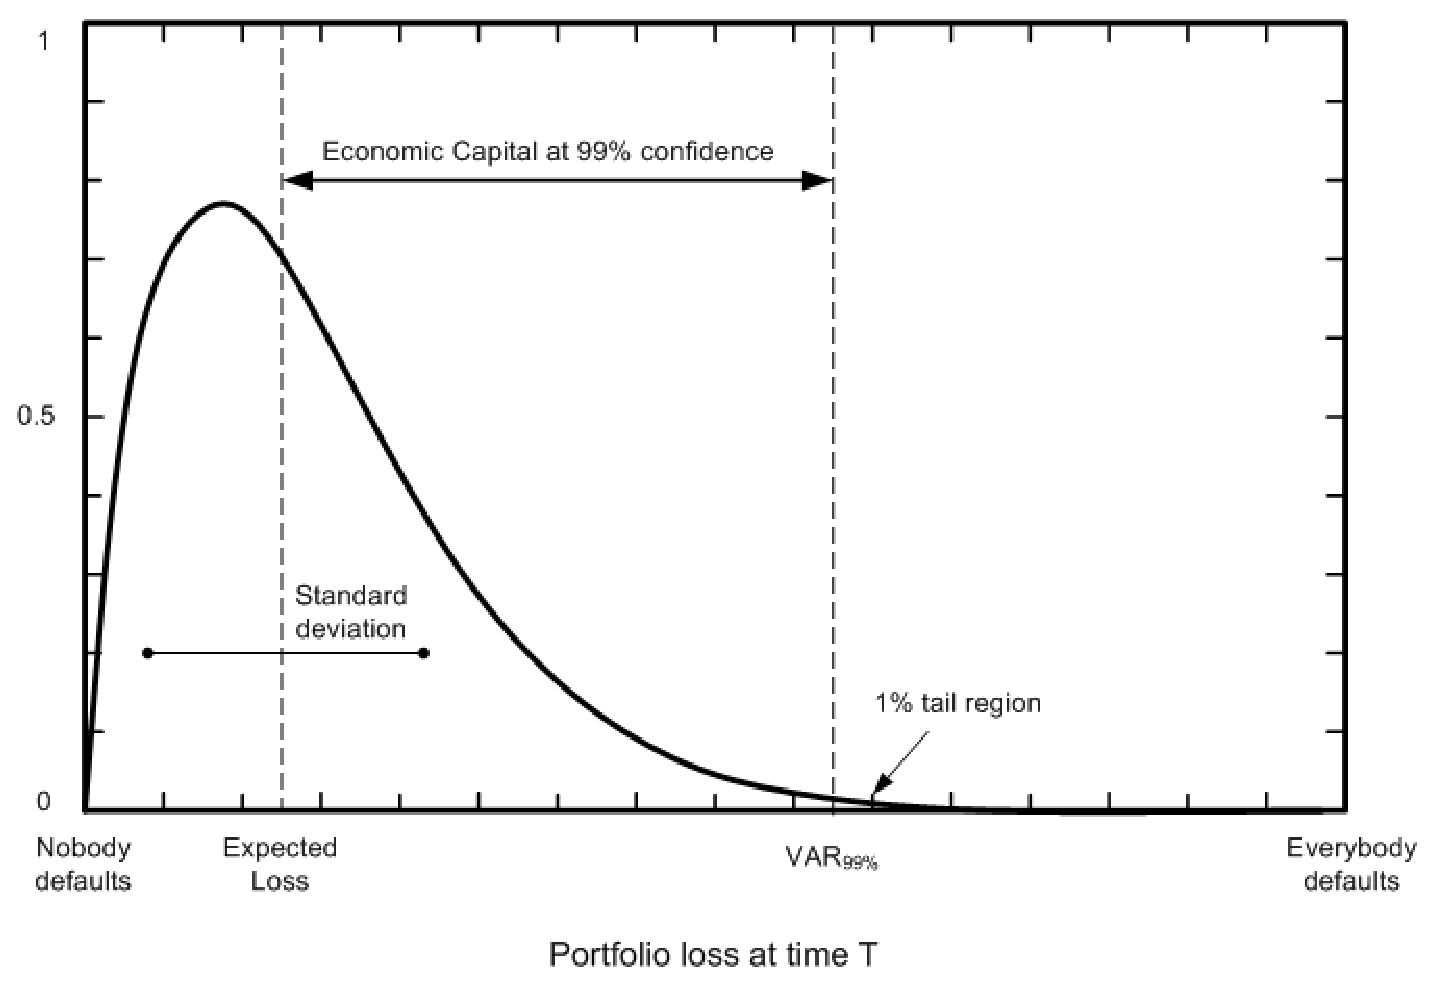
\includegraphics[height=7cm, angle=0]{./images/creditvar.eps}
\caption{Portfolio value at time $T$}
\label{creditvar}
\end{center}
\end{figure}

\paragraph{Ejemplo.} Calculemos el VAR de una cartera de cr\'editos
sencilla, de la que se puede obtener la distribuci\'on de las p\'erdidas de
forma expl\'icita. Sea una cartera de $1$ solo sector con $100$ clientes sin
correlaci\'on alguna entre ellos. Cada cliente tiene un activo que consiste en
devolver $1$ \euro~ al cabo de $T$ tiempo. Supongamos que el sistema de ratings
solamente contempla $2$ categor\'ias crediticias, no-Default y Default. La
probabilidad de hacer fallido al cabo de 1 a\~no es $0.1$.
\newline
\newline
En este caso, se puede modelar la p\'erdida provocada por el impago del cliente
$i$ al cabo de 1 a\~no como una variable aleatoria Bernouilli, $X_i \sim Ber(0.1)$.
La p\'erdida de la cartera al cabo de 1 a\~no es la suma de las p\'erdidas de
cada cliente, $Z = \sum_{i=1}^{100} X_i$, que por definici\'on es una
variable aleatoria Binomial, $Z \sim B(100,0.1)$.
\newline
\newline
La P\'erdida Esperada al cabo de 1 a\~no es
\begin{displaymath}
\textrm{Expected Loss} = E(Z) = 10
\end{displaymath}

El VAR al nivel de confianza $99\%$ al cabo de 1 a\~no es:
\begin{displaymath}
VAR_{99\%} = \textrm{inf}\{z | F_Z(z) \geq 99\%\}
\end{displaymath}
Expresado en t\'erminos de la funci\'on de densidad
\begin{displaymath}
P(Z \leq VAR_{99\%}) = 99\%
\end{displaymath}
Consultamos las tablas cdf de la Binomial(100,0.1)
\begin{displaymath}
P(Z \leq 17) = 98.99927\%
\end{displaymath}
Por tanto, podemos considerar que $VAR_{99\%}$ es
\begin{displaymath}
\textrm{VAR}_{99\%} = 17
\end{displaymath}

El TCE al nivel de confianza $99\%$ al cabo de 1 a\~no es:
\begin{displaymath}
TCE_{99\%} = E(Z | Z > VAR_{99\%}(Z))
\end{displaymath}
Equivalentemente
\begin{displaymath}
TCE_{99\%} = \frac{\sum_{i=18}^{100} i\cdot P(Z=i)}{\sum_{i=18}^{100} P(Z=i)} = 18.78458
\end{displaymath}

El Capital Econ\'omico al nivel de confianza $99\%$ al cabo de 1 a\~no es:
\begin{displaymath}
\textrm{Economic Capital}_{99\%}(Z) = \textrm{VAR}_{99\%}(Z) - E(Z) = 17 - 10 = 7
\end{displaymath}

Este ejemplo no es significativo debido a que se han realizado dos supuestos
que en el mundo real no se cumplen: todos los creditores se modelan de la misma 
forma y los fallidos son independientes. Se obtiene que la distribuci\'on de las 
p\'erdidas de la cartera al cabo de 1 a\~no es una variable aleatoria Binomial(100,0.1),
que puede ser aproximada de forma precisa por una Normal(10,9). Esto no concuerda
con las observaciones reales, que muestran que la distribuci\'on de las p\'erdidas
es fuertemente asim\'etrica respecto a la p\'erdida esperada.



%***************************************************************************
%
% CreditCruncher - A portfolio credit risk valorator
% Copyright (C) 2004 Gerard Torrent
%
% This program is free software; you can redistribute it and/or
% modify it under the terms of the GNU General Public License
% as published by the Free Software Foundation; either version 2
% of the License.
%
% This program is distributed in the hope that it will be useful,
% but WITHOUT ANY WARRANTY; without even the implied warranty of
% MERCHANTABILITY or FITNESS FOR A PARTICULAR PURPOSE.  See the
% GNU General Public License for more details.
%
% You should have received a copy of the GNU General Public License
% along with this program; if not, write to the Free Software
% Foundation, Inc., 59 Temple Place - Suite 330, Boston, MA 02111-1307, USA.
%
%
% resolution.tex - TeX documentation file - $Rev$
% --------------------------------------------------------------------------
%
% 2005/01/22 - Gerard Torrent [gerard@fobos.generacio.com]
%   . initial release
%
% 2005/10/15 - Gerard Torrent [gerard@fobos.generacio.com]
%   . added Rev (aka LastChangedRevision) svn tag
%
%***************************************************************************

\chapter{Resoluci\'on}
\label{sec:resolution}

\section{Esquema general}

El m\'etodo de resoluci\'on implementado por CreditCruncher consiste en
aplicar el m\'etodo de Monte Carlo. En la figura \ref{fig:esquema1} se
muestra el esquema de un paso del m\'etodo de Monte Carlo.

\begin{figure}[!hb]
\begin{center}
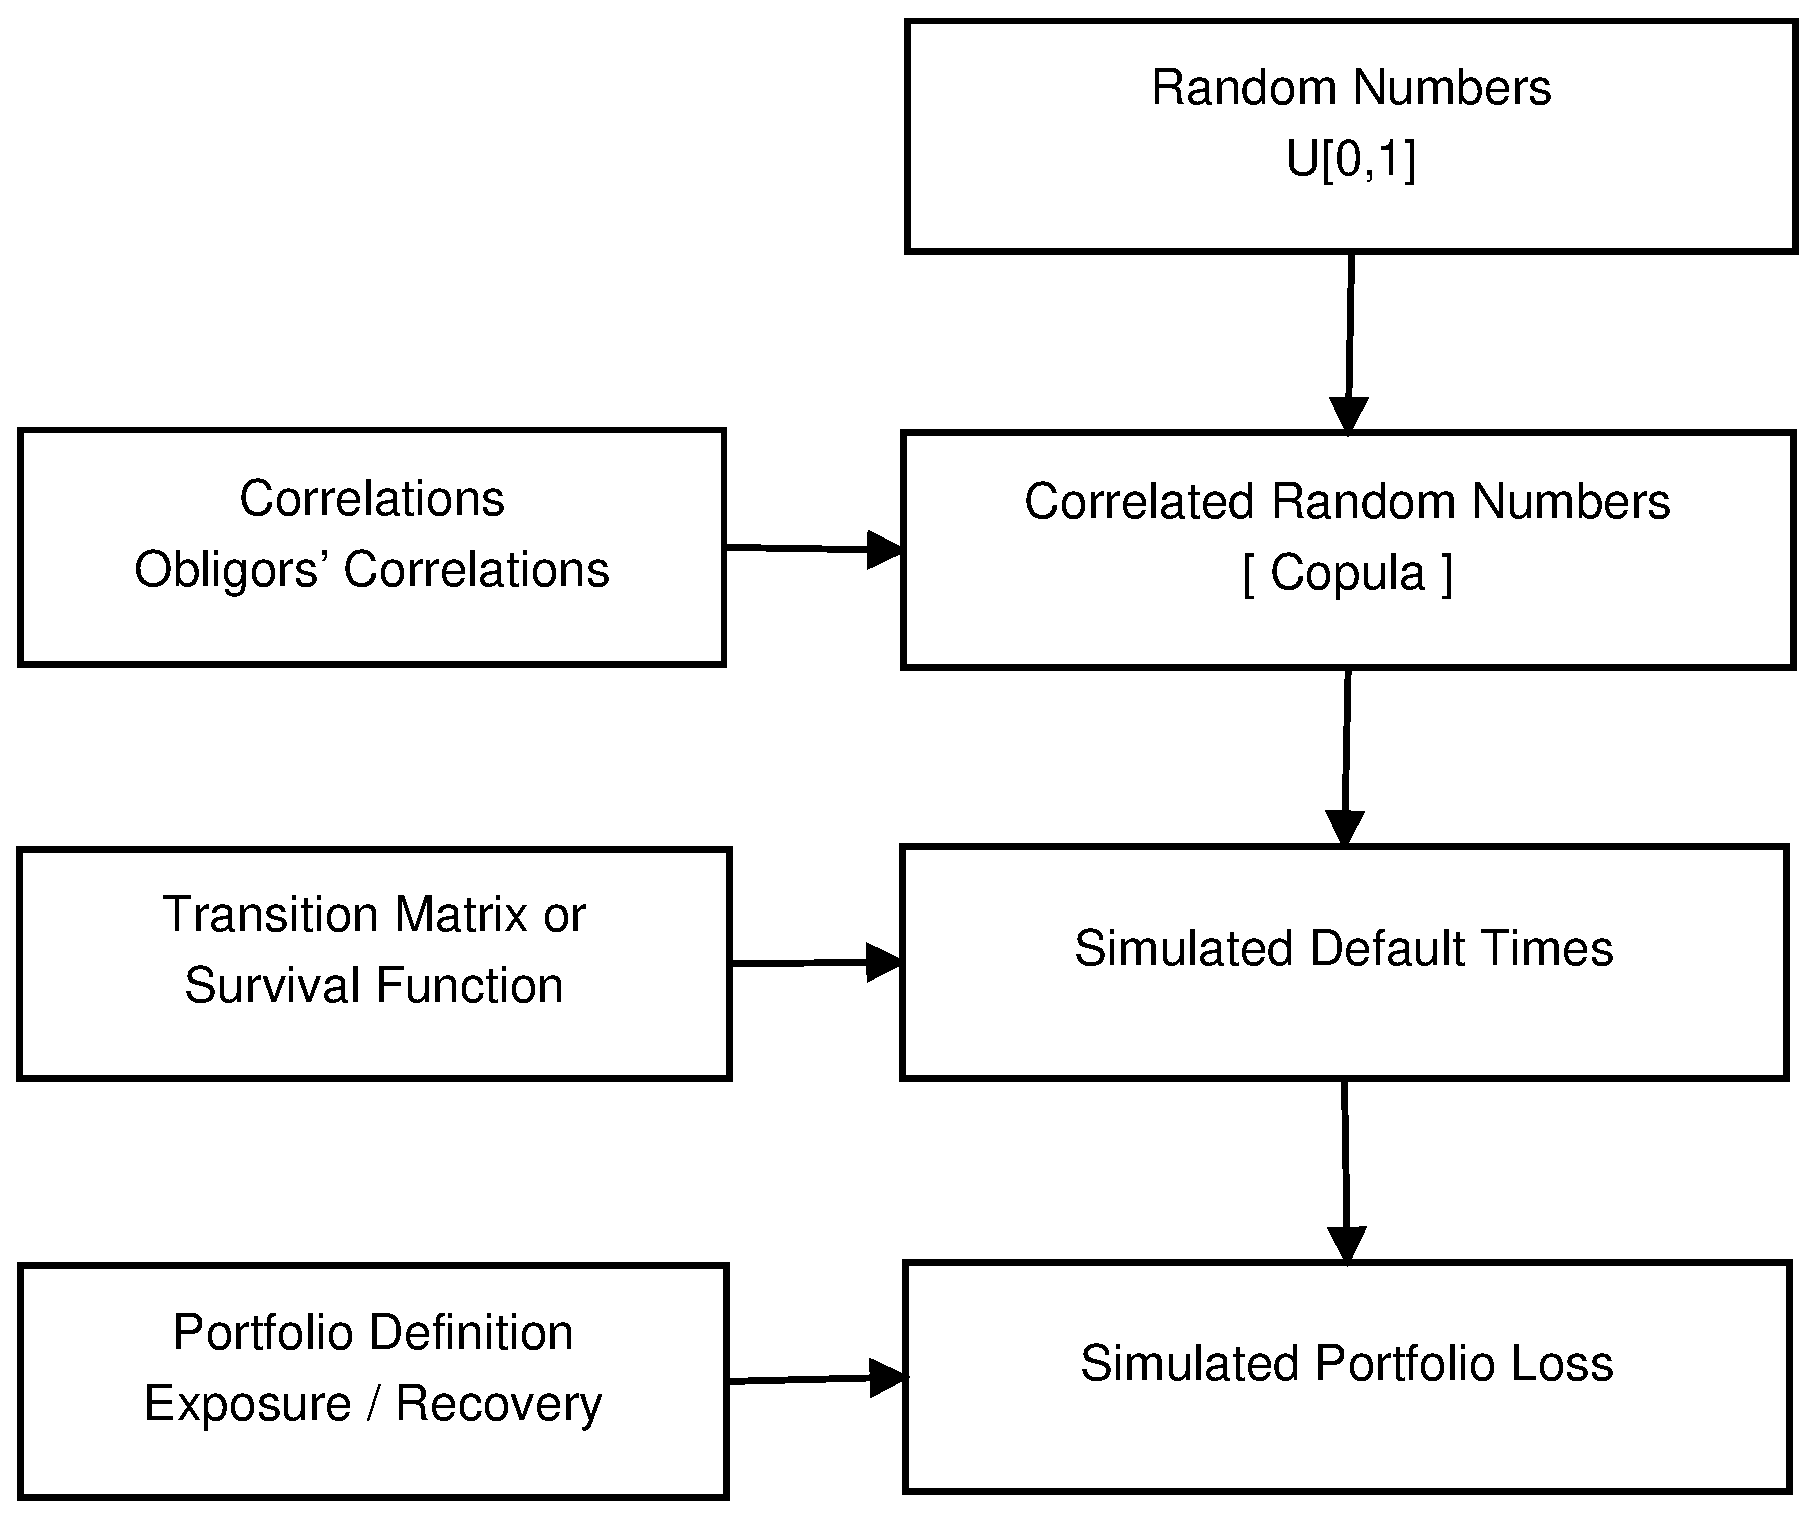
\includegraphics[width=10cm,angle=0]{./images/esquema1.eps}
\caption{Esquema de la simulaci\'on}
\label{fig:esquema1}
\end{center}
\end{figure}

%---------------------------------------------------------------------------

\section{El m\'etodo de Monte Carlo}

Se recomienda la lectura de la referencia \cite{mc:mervyn}. Se trata de los 
apuntes para una clase del profesor Mervyn Marasinghe. Se expone el m\'etodo 
de Monte Carlo y las t\'ecnicas de reducci\'on de la varianza.

\paragraph{Definici\'on.} Dado un conjunto de observaciones, $x_1, \cdots, x_N$,
de la variable aleatoria $X$, definimos la \emph{funci\'on de distribuci\'on emp\'irica}
\index{Funci\'on de distribuci\'on emp\'irica} como:
\begin{displaymath}
\widetilde{F_X(y)} = \frac{1}{N} \sum_{i=1}^{N} I_{(-\infty,y]}(x_i) \qquad
I_{(-\infty,y]}(x) = \left\{
\begin{array}{ll}
1 & \textrm{ if } x \in (-\infty,y] \cr
0 & \textrm{ otherwise}
\end{array}
\right.
\end{displaymath}

\paragraph{Proposici\'on.} La funci\'on de distribuci\'on emp\'irica tiende a 
la funci\'on de distribuci\'on al incrementar el n\'umero de observaciones.
\begin{displaymath}
\qquad \lim_{n\to\infty} \widetilde{F_X} = F_X
\end{displaymath}

\paragraph{Definici\'on.} Sea $X$ una variable aleatoria con funci\'on de 
distribuci\'on conocida, $F$. El \emph{m\'etodo de Monte Carlo}\index{M\'etodo
de Monte Carlo} consiste en obtener la funci\'on de distribuci\'on emp\'irica 
de la variable aleatoria $H(X)$ usando el siguiente m\'etodo:
\begin{displaymath}
\begin{array}{ccc}
F_X                 &     \quad       & \widetilde{F_{H(X)}}    \cr
\downarrow          &     \quad       & \uparrow                \cr
\textrm{simulation} &     \quad       & \textrm{empirical } cdf \cr
\downarrow          &     \quad       & \uparrow                \cr
x_1,\cdots,x_N      & \longrightarrow & H(x_1),\cdots,H(x_N)
\end{array}
\end{displaymath}

\paragraph{Observaci\'on.} Problemas aparentemente no relacionados con las 
variables aleatorias pueden reformularse como un problema donde intervenga
una variable aleatoria y ser resueltos por el m\'etodo de Monte Carlo. 
Normalmente se formula el problema original como el c\'alculo de un 
estad\'istico (pe. la media) sobre la funci\'on de distribuci\'on. Al
m\'etodo de Monte Carlo se le atribuye una velocidad de convergencia  
del orden de $1/\sqrt{N}$.

\paragraph{Ejemplo:} El ejemplo cl\'asico es obtener el valor de la integral 
de la funci\'on $W$ entre $0$ y $1$. Lo reformulamos de la siguiente forma:
\begin{displaymath}
\int_{0}^{1} W(u) du = \int_{0}^{1} W(u) \phi(u) du = E[W(U)]
\end{displaymath}
donde $U \sim U[0,1]$ y $\phi(u) = \textrm{pdf}(U) = 1$. La \'ultima igualdad se
establece usando la preposici\'on enunciada en el ap\'endice \ref{apendix:stats}.
Finalmente la integral se aproxima calculando la media de un conjunto de puntos
con distribuci\'on $W(U)$.

%---------------------------------------------------------------------------

\section{Variables aleatorias correlacionadas}

Se recomienda la lectura de las referencias \cite{copu:wang} y 
\cite{copu:pitfalls}. Se trata de art\'iculos donde se explica que es una 
c\'opula, sus propiedades, como simularlas, creencias err\'oneas, etc.

\paragraph{Definici\'on.} Llamamos \emph{c\'opula}\index{C\'opula} a la funci\'on
de distribuci\'on de una variable aleatoria $n$-dimensional tal que sus distribuciones
marginales \index{Distribuciones marginales} son variables aleatorias $U[0,1]$.
\begin{displaymath}
C(u_1, \cdots,u_n)=P(U_1 \leq u_1, \cdots, U_n \leq u_n) \qquad U_k \sim U[0,1]
\end{displaymath}

\begin{figure}[!hb]
\begin{minipage}[c]{0.5\columnwidth}%
  \centering
  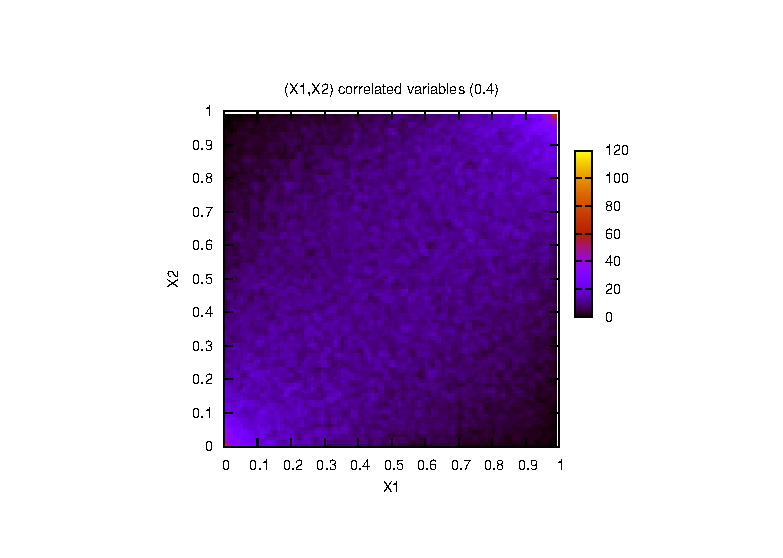
\includegraphics[height=5cm, angle=0]{./images/copula.eps}
\end{minipage}%
\hfill{}
\begin{minipage}[c]{0.5\columnwidth}%
  \centering
  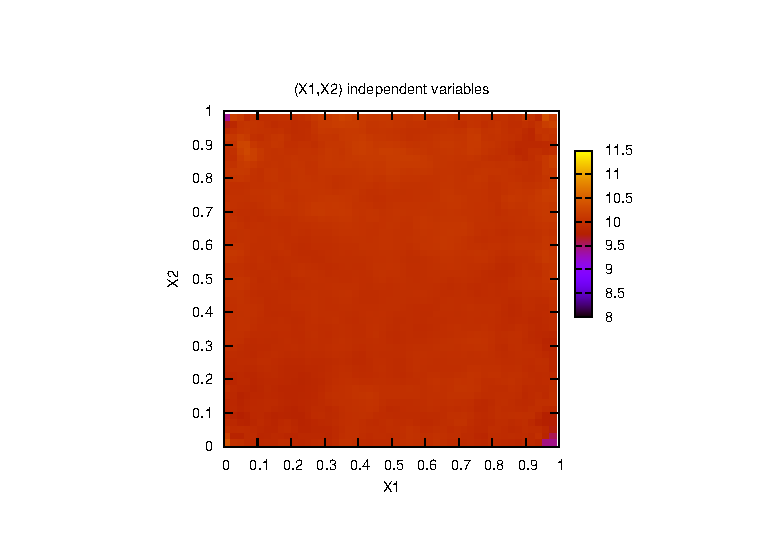
\includegraphics[height=5cm, angle=0]{./images/uniform.eps}
\end{minipage}%
\caption{Bivariate distribution plot with correlated and uncorrelated variables}
\label{copulas}
\end{figure}

\paragraph{Teorema.} \index{Teorema de Sklar} Toda variable aleatoria $n$-dimensional
puede separarse en las distribuciones seguidas por sus componentes (las distribuciones
marginales) y una c\'opula. Sea $F$ una funci\'on de distribuci\'on $n$-dimensional y
$f_1,\cdots, f_n$ sus marginales. El teorema de Sklar asegura que existe una 
c\'opula $C$ tq.
\begin{displaymath}
F(x_1, \cdots,x_n) = C(f_1(x_1), \cdots, f_n(x_n)) 
\end{displaymath}

\paragraph{Observaci\'on.} Una variable aleatoria $n$-dimensional no est\'a 
determinada por sus marginales y correlaciones entre estas. Dicho de otra
forma, existen infinitas formas de combinar las distribuciones marginales
 a trav\'es de c\'opulas de forma que cumplan las correlaciones. Las distribuciones 
el\'ipticas (que incluyen la distribuci\'on multinomial) son una excepci\'on. 

%---------------------------------------------------------------------------

\section{Simulaci\'on del tiempo de fallido}

El objetivo de este apartado es proporcionar m\'etodos para simular los
tiempos de fallido, $\vec{t_w} = (t_w^1,t_w^2,t_w^3,\cdots,t_w^{nc})$ de los
clientes cumpliendo:
\begin{itemize}
\item los fallidos de cada cliente deben satisfacer la matriz de transici\'on $M_T$
(o la funci\'on de supervivencia, $Survival(r,t)$).
\item la correlaci\'on entre los fallidos de los clientes debe cumplir la matriz
de correlaci\'on entre clientes, $\Theta$
\end{itemize}

\subsection{M\'etodo Rating-Path}
\label{res:mrt}
\index{M\'etodo Rating-Path}

Este m\'etodo simula la evoluci\'on del rating del cliente a lo largo del tiempo.
El tiempo de fallido se obtiene al alcanzar el rating $Default$. Para este m\'etodo
es necesario disponer de la matriz de transici\'on, $M_T$.

\paragraph{Paso 1.} Segmentamos el tiempo en intervalos constantes de forma que
el intervalo de tiempo entre $t_i$ y $t_{i+1}$ es el cubierto por la matriz de
transici\'on, $T$.
\begin{displaymath}
t_0,t_1,t_2,\cdots,t_k, \cdots
\end{displaymath}

\paragraph{Paso 2.} Para cada intervalo de tiempo $k$ creamos una c\'opula,
$Qk$ de dimensi\'on $nc$ que satisfaga la matriz de correlaci\'on entre
clientes, $\Theta$.
\begin{displaymath}
Q_1, Q_2, Q_3, \cdots, Q_k, \cdots
\end{displaymath}

\paragraph{Paso 3.} Simulamos las c\'opulas $Q_1, Q_2, Q_3, \cdots, Q_k, \cdots$.
Cada realizaci\'on de $Q_k$ consiste en un vector de componentes
$(Q_k(1), Q_k(2), \cdots, Q_k(nc))$.

\paragraph{Paso 4.} Simulamos el rating del cliente $i$ en $t_1$ de la forma siguiente:
disponemos del rating inicial $rating(i,t_0)$ y un valor $Q_1(i) \in [0,1]$
proporcionado por el componente $i$-\'esimo de $Q_1$. Entonces
\begin{displaymath}
rating(i,t_1) = M_T^{-1}(rating(i,t_1),Q_1(i))
\end{displaymath}
Este paso se encuentra ilustrado en la figura \ref{simrp}.

\paragraph{Paso 5.} Simulamos el rating del cliente $i$ en $t_k$ de la forma siguiente:
disponemos del rating anterior $rating(i,t_{k-1})$ y un valor $Q_k(i) \in [0,1]$
proporcionado por el componente $i$-\'esimo de $Q_k$. Entonces
\begin{displaymath}
rating(i,t_k) = M_T^{-1}(rating(i,t_{k-1}),Q_k(i))
\end{displaymath}
Este paso se encuentra ilustrado en la figura \ref{simrp}. Finalmente, aproximamos
el tiempo de fallido del cliente $i$ de la siguiente forma:
\begin{displaymath}
t_w^i = inf\{t_k | rating(i,t_k) = Default\}
\end{displaymath}

\begin{figure}[!hb]
\begin{center}
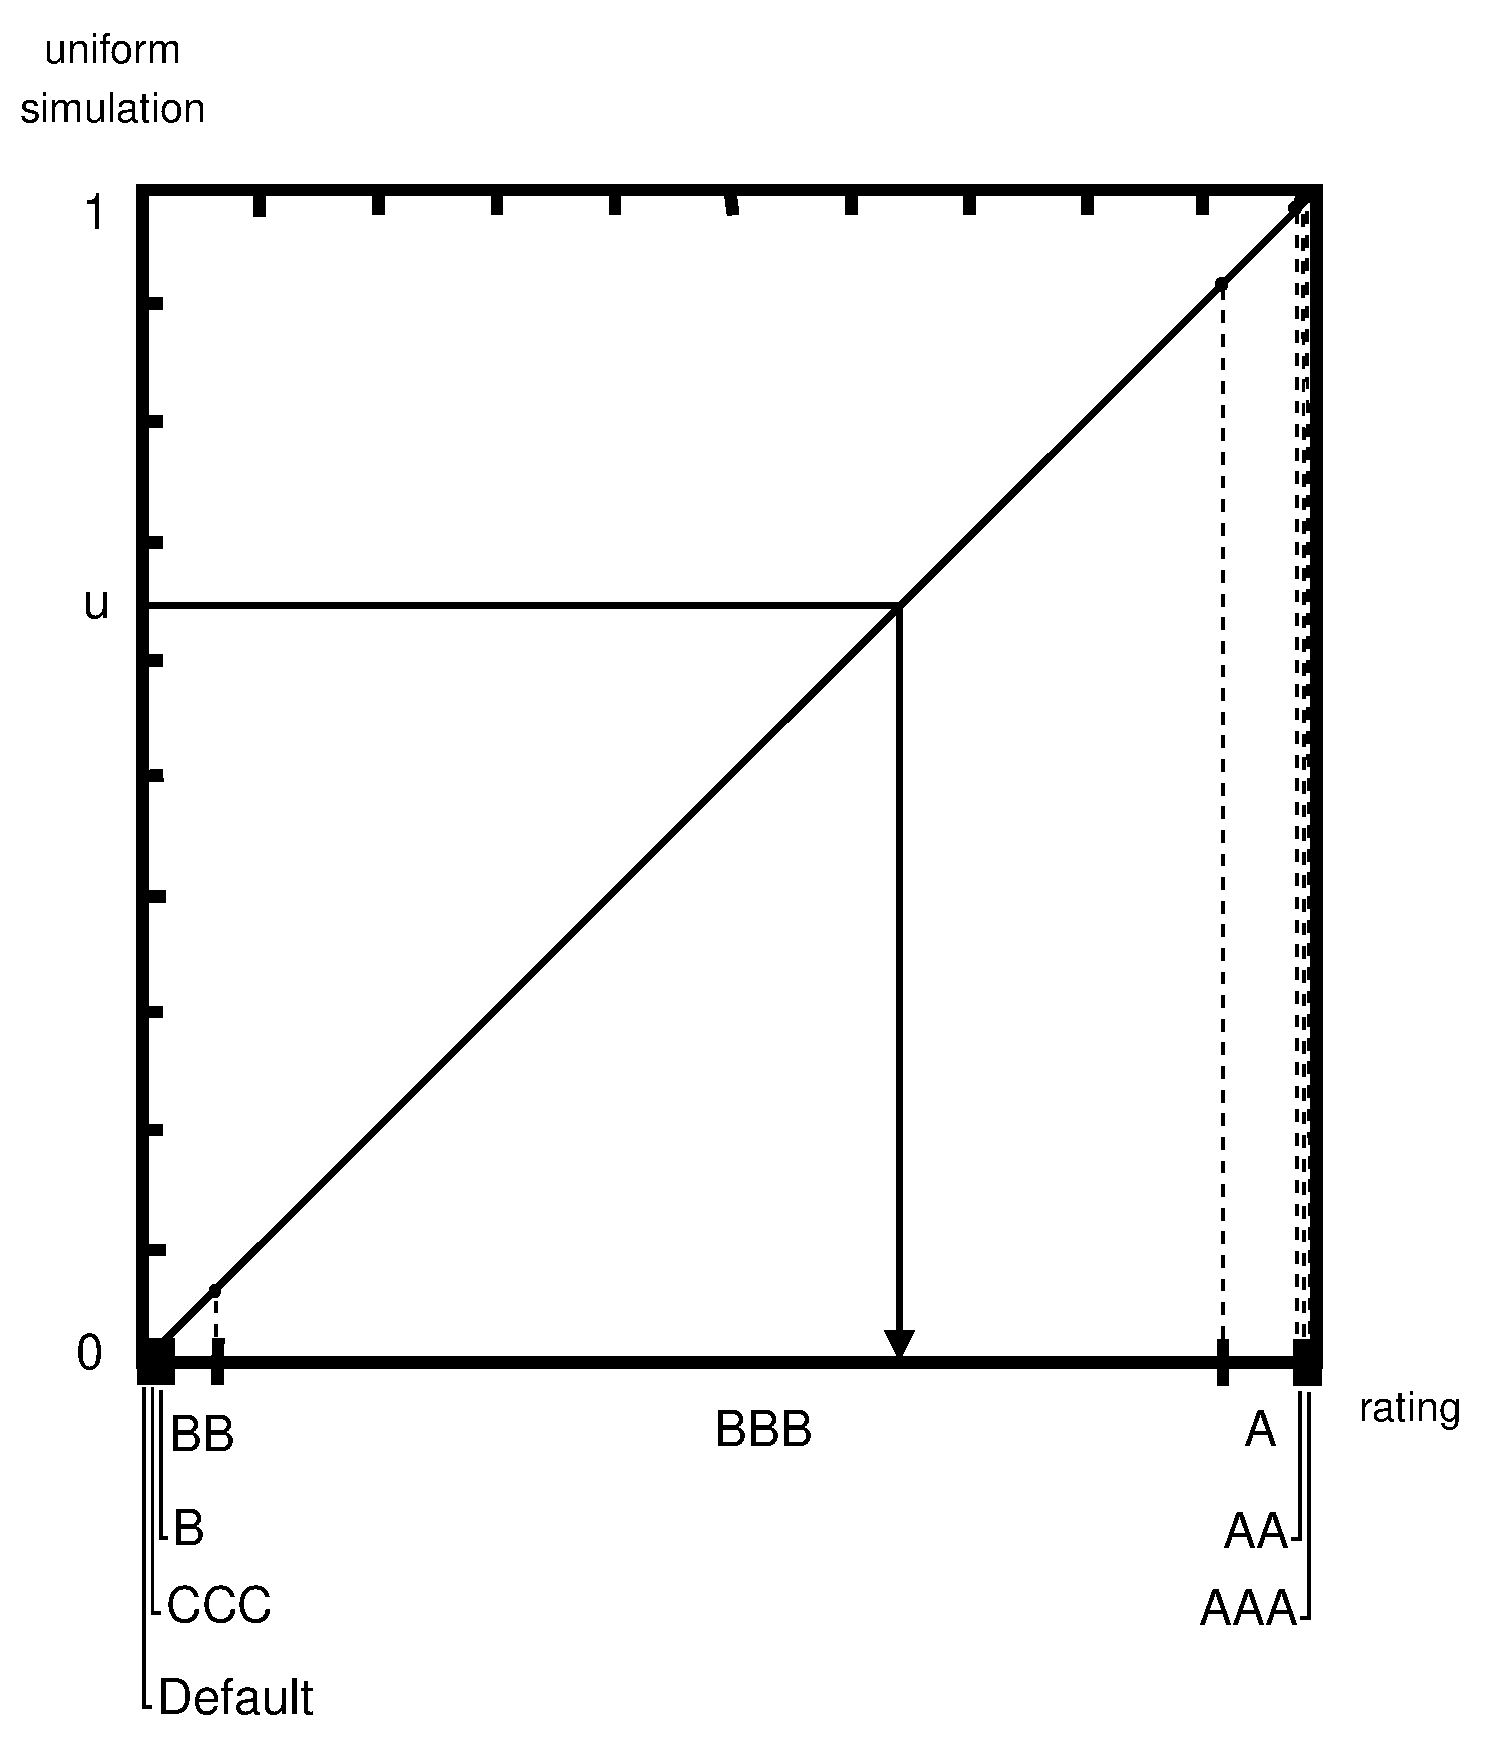
\includegraphics[width=7cm,angle=0]{./images/simrp.eps}
\caption{Simulaci\'on de la evoluci\'on del rating $BBB$ a $T$ tiempo}
\label{simrp}
\end{center}
\end{figure}

\subsection{M\'etodo Time-To-Default}
\label{res:mttd}
\index{M\'etodo Time-To-Default}

Este m\'etodo consiste en simular directamente el tiempo de fallido de los
clientes. Requiere disponer de la funci\'on de supervivencia. En caso
de disponer solamente de la matriz de transici\'on puede calcularse la funci\'on
de supervivencia asociada a la matriz de transici\'on usando las f\'ormulas
\ref{eq:survival1} y \ref{eq:cdfr1}.

\paragraph{Paso 1.} Creamos una c\'opula de dimensi\'on $nc$ que satisfaga la
matriz de correlaci\'on entre clientes, $\Theta$.
\begin{displaymath}
Q
\end{displaymath}

\paragraph{Paso 2.} Simulamos la c\'opula $Q$. La realizaci\'on de $Q$ consiste
en un vector de componentes $(Q(1), Q(2), \cdots, Q(nc))$.

\paragraph{Paso 2.} Simulamos el tiempo de fallido del cliente $i$ de la forma siguiente:
disponemos del rating inicial, $rating(i,t_0)$ y un valor $Q(i) \in [0,1]$ proporcionado
por el componente $i$-\'esimo de $Q$. Entonces:
\begin{displaymath}
t_w^i = Survival^{-1}(rating(i,t_0),Q(i))
\end{displaymath}
Este paso se encuentra ilustrado en la figura \ref{simttd}.

\begin{figure}[!hb]
\begin{center}
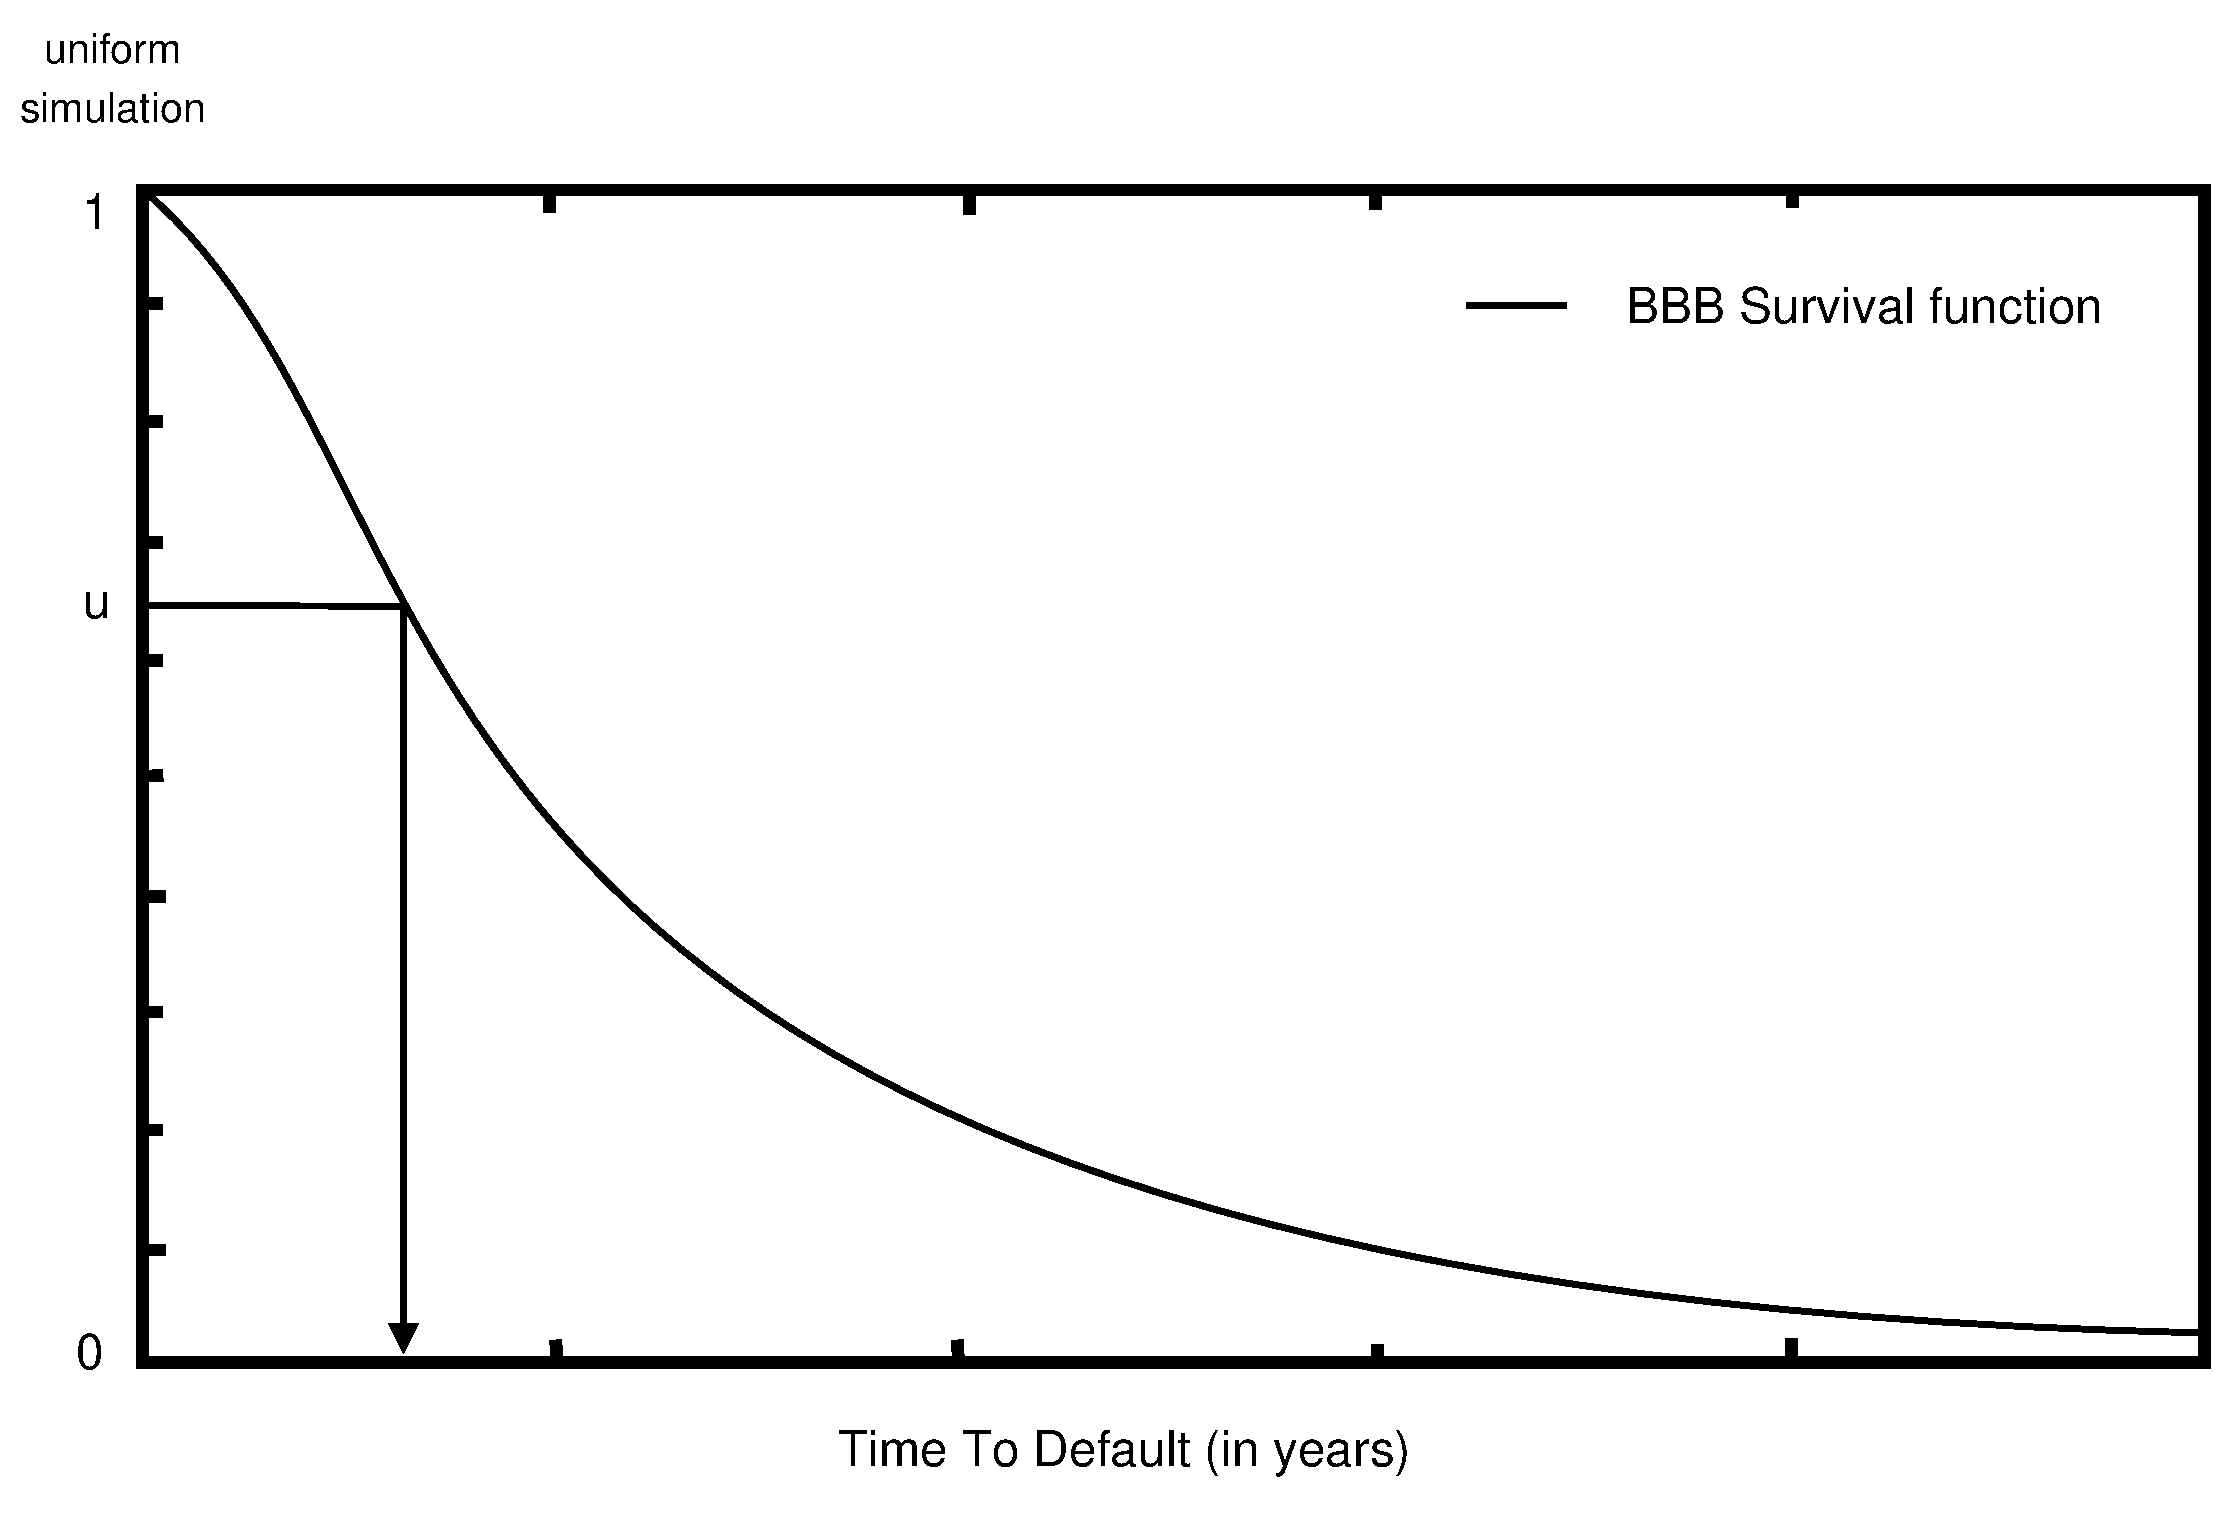
\includegraphics[width=10cm,angle=0]{./images/simttd.eps}
\caption{Simulaci\'on del tiempo hasta el fallido del rating $BBB$}
\label{simttd}
\end{center}
\end{figure}

%---------------------------------------------------------------------------

\section{Evaluaci\'on de la cartera}

En las definiciones siguientes se considera que $S$ es la curva spot en $t_0$,
$na_i$ es el n\'umero de activos del cliente $i$ y $nc$ el n\'umero de clientes.
Asimismo se considera que el casflow y netting de cada activo est\'a fijado y
no depende de la evoluci\'on del cliente.

\paragraph{Definici\'on.} Definimos el valor del activo $j$ del cliente $i$
evaluado en $t_K$ entre el tiempo $t_0$ y $t_K$, habiendo hecho fallido en
tiempo $t_w$ como:
\begin{equation}
X_{i,j}(t_w;t_0,t_K) = 
\end{equation}
\begin{displaymath}
\textrm{1}_{[t_w \leq t_K]} \cdot \textrm{netting}(t_w) \cdot \Upsilon_S(t_w,t_K) + 
\sum_{t=t_0}^{t_K} \textrm{1}_{[t < t_w]} \cdot \textrm{cashflow}(t) \cdot \Upsilon_S(t,t_K)
\end{displaymath}

\paragraph{Definici\'on.} Definimos el valor de los activos del cliente $i$
evaluados en $t_K$ entre el tiempo $t_0$ y $t_K$, habiendo hecho fallido en
tiempo $t_w$ como:
\begin{equation}
X_i(t_w;t_0,t_K) = \sum_{j=0}^{na_i} X_{i,j}(t_w;t_0,t_K)
\end{equation}

\paragraph{Definici\'on.} Definimos el valor de la cartera evaluada en $t_K$
entre el tiempo $t_0$ y $t_K$, siendo $\vec{t_w}$ los tiempos en los que han hecho
fallido los clientes como:
\begin{equation}
X(\vec{t_w};t_0,t_K) = \sum_{i=0}^{nc} X_i(t_w^i;t_0,t_K) =
\sum_{i=0}^{nc} \sum_{j=0}^{na_i} X_{i,j}(t_w^i;t_0,t_K)
\end{equation}

\paragraph{Definici\'on.} Definimos las p\'erdidas de la cartera evaluada en $t_K$
entre el tiempo $t_0$ y $t_K$, siendo $\vec{t_w}$ los tiempos en los que han hecho
fallido los clientes como:
\begin{equation}
Z(\vec{t_w};t_0,t_K) = X(\vec{t_\infty};t_0,t_K) - X(\vec{t_w};t_0,t_K)
\end{equation}

%---------------------------------------------------------------------------

\section{Valoraci\'on del riesgo}
\label{res:risk}

El m\'etodo de Monte Carlo genera $N$ realizaciones, $\{z_1,z_2,z_3,\cdots,z_N\}$,
de la variable aleatoria $Z$ (p\'erdidas de la cartera) que permiten obtener la
funci\'on de distribuci\'on emp\'irica. A continuaci\'on se exponen los estad\'isticos
calculados, sus estimaciones y el intervalo de confianza al nivel de confianza $\alpha$.
CreditCruncher utiliza el entorno \emph{R} \footnote{http://www.r-project.org} para realizar
los c\'alculos estad\'isticos. Para mas informaci\'on acerca de \emph{R} v\'ease \cite{stats:R}.
Sea $\phi^{-1}(x)$ la inversa de la funci\'on de distribuci\'on de la Normal(0,1).

\paragraph{Expected Loss.}\index{Expected Loss} F\'ormula extra\'ida de \cite{stats:schaum}
basada en el teorema del l\'imite central.
\begin{displaymath}
\mu_Z = \widehat{\mu_Z} \pm \phi^{-1}\left(\frac{1-\alpha}{2}\right) \cdot \frac{\widehat{\sigma_Z}}{\sqrt{N}}
\end{displaymath}
Consulte \ref{apendix:estim} para el c\'alculo de $\widehat{\mu_Z}$ y $\widehat{\sigma_Z}$.

\paragraph{Desviaci\'on est\'andar.}\index{Desviaci\'on Est\'andar} F\'ormula extra\'ida de
\cite{stats:schaum} basada en el teorema del l\'imite central.
\begin{displaymath}
\sigma_Z = \widehat{\sigma_Z} \pm \phi^{-1}\left(\frac{1-\alpha}{2}\right) \cdot \frac{\widehat{\sigma_Z}}{\sqrt{2N}}
\end{displaymath}
Consulte \ref{apendix:estim} para el c\'alculo de $\widehat{\sigma_Z}$.

\paragraph{Value at Risk.}\index{Value At Risk} Fijado un nivel de $VAR = x$
\begin{displaymath}
VAR_{x}(Z) = \widehat{q_{x}(Z)} \pm \phi^{-1}\left(\frac{1-\alpha}{2}\right) \cdot \textrm{stderr}(q_{x}(Z))
\end{displaymath}
Consulte \ref{apendix:estim} y \ref{apendix:stderrvar} para el c\'alculo de
$\widehat{q_{x}(Z)}$ y $\textrm{stderr}(q_{x}(Z))$.

\paragraph{TCE o Expected Shortfall.}\index{Tail Conditional Expectation}\index{Expected Shortfall}
Fijado un nivel de $VAR = x$
\begin{displaymath}
TCE_{x}(Z) = \widehat{TCE_{x}(Z)} \pm \phi^{-1}\left(\frac{1-\alpha}{2}\right) \cdot \textrm{stderr}(TCE_{x}(Z))
\end{displaymath}
Consulte \ref{apendix:estim} y \ref{apendix:stderrtce} para el c\'alculo de
$\widehat{TCE_{x}(Z)}$ y $\textrm{stderr}(TCE_{x}(Z))$.


%***************************************************************************
%
% CreditCruncher - A portfolio credit risk valorator
% Copyright (C) 2004 Gerard Torrent
%
% This program is free software; you can redistribute it and/or
% modify it under the terms of the GNU General Public License
% as published by the Free Software Foundation; either version 2
% of the License.
%
% This program is distributed in the hope that it will be useful,
% but WITHOUT ANY WARRANTY; without even the implied warranty of
% MERCHANTABILITY or FITNESS FOR A PARTICULAR PURPOSE.  See the
% GNU General Public License for more details.
%
% You should have received a copy of the GNU General Public License
% along with this program; if not, write to the Free Software
% Foundation, Inc., 59 Temple Place - Suite 330, Boston, MA 02111-1307, USA.
%
%
% implementation.tex - TeX documentation file
% --------------------------------------------------------------------------
%
% 2005/01/22 - Gerard Torrent [gerard@fobos.generacio.com]
%   . initial release
%
%***************************************************************************

\chapter{Implementaci\'on de la soluci\'on}
\label{sec:implementation}

\section{Generaci\'on de c\'opulas}

TODO: descripci\'on del proceso de generacion de copulas normales

\section{Simulaci\'on de productos}

TODO: listado de los productos soportados y descripci\'on del proceso de 
simulaci\'on seguido.


\section{Proceso de agregaci\'on}

TODO: descripcion de los agregadores y metodo usado para evitar recalculo 
de los activos en cada simulacion + Agregaci\'on de productos


\section{Dimensiones del problema}

TODO: Estimaciones de uso de memoria, estimaci\'on del numero de operaciones,
estimacion del tiempo de computo


\section{Convergencia de la soluci\'on}

TODO: N\'úmero de iteraciones necesarias, aceleraci\'on de la convergencia
usando metodología antitetic


\appendix

%***************************************************************************
%
% CreditCruncher - A portfolio credit risk valorator
% Copyright (C) 2004 Gerard Torrent
%
% This program is free software; you can redistribute it and/or
% modify it under the terms of the GNU General Public License
% as published by the Free Software Foundation; either version 2
% of the License.
%
% This program is distributed in the hope that it will be useful,
% but WITHOUT ANY WARRANTY; without even the implied warranty of
% MERCHANTABILITY or FITNESS FOR A PARTICULAR PURPOSE.  See the
% GNU General Public License for more details.
%
% You should have received a copy of the GNU General Public License
% along with this program; if not, write to the Free Software
% Foundation, Inc., 59 Temple Place - Suite 330, Boston, MA 02111-1307, USA.
%
%
% appendices.tex - TeX documentation file
% --------------------------------------------------------------------------
%
% 2005/01/22 - Gerard Torrent [gerard@fobos.generacio.com]
%   . initial release
%
%***************************************************************************

\chapter{Ap\'endices}
\label{sec:apendixes}

%---------------------------------------------------------------------------

\section{Conceptos b\'asicos de estad\'istica}


%---------------------------------------------------------------------------

\section{C\'alculo de la raiz de una matriz}

\paragraph{Definici\'on.}
Diremos que 2 matrices $A$ y $B$ de orden $n$ son semejantes si existe una 
matriz, $P$, de orden $n$ con $det(P) \neq 0$ tal que 
$B = P^{-1} \cdot A \cdot P$.


\paragraph{Proposici\'on.} Si dos matrices $A$ y $B$ son semejantes 
($B = P^{-1} \cdot A \cdot P$) entonces:
\begin{displaymath}
det(A) = det(B)
\end{displaymath}
\begin{displaymath}
B^n = P^{-1} \cdot A^{n} \cdot P
\end{displaymath}

\paragraph{Definici\'on.} 
Diremos que Una matriz $A$ de orden $n$ es diagonalizable si es semejante a una 
matriz diagonal $D$, o sea, $A = P^{-1} \cdot D \cdot P$ siendo $det(D) \neq 0$.

\paragraph{Proposici\'on.} 
Para que una matriz $A$ sea diagonalizable es necesario y suficiente que:
\begin{itemize}
\item Los valores propios de $A$ sean todos reales
\item Los $n$ vectores propios de $A$ sean independientes
\end{itemize}

\paragraph{Proposici\'on.}
Si una matriz $A$ es diagonalizable ($A = P^{-1} \cdot D \cdot P$) entonces: 
\begin{itemize}
\item $D$ es una matriz diagonal compuesta por los valores propios de la matriz $A$
\item $P$ es la matriz formada por los vectores propios de la matriz $A$
\end{itemize}

\paragraph{Resultado.}
Sea $A$ la ra\'iz $n$-esima de una matriz diagonalizable $B$. Entonces:
\begin{displaymath}
A^n = B = P^{-1} \cdot D \cdot P 
\Longrightarrow  
A = \sqrt[n]{B} = P^{-1} \cdot \sqrt[n]{D} \cdot P
\end{displaymath} 

%---------------------------------------------------------------------------

\section{La variable aleatoria de Bernoulli}

\subsection{Definici\'on y propiedades}

\subsection{Simulaci\'on}

TODO: ampliarla al caso x1, ..., xn. simulacion usando uniforme [0,1] + etc.

%---------------------------------------------------------------------------

\section{La variable aleatoria normal}

\subsection{Definici\'on y propiedades}

\begin{displaymath}
P(X \leq x) = \Phi(x) = \int_{-\infty}^{x} \frac{e^{-t^2}}{\sqrt{2 \pi}} dt
\end{displaymath}

\subsection{Simulaci\'on}

Para la generaci\'on de una realizaci\'on, $z$, de una variable aleatoria normal  
$Z \sim N(\mu, \sigma)$ utilizamos el siguiente algoritmo:

\begin{displaymath}
z = \mu + \sigma\cdot \sqrt{-2 \cdot ln(u[0,1])} \cdot cos(2 \cdot \pi \cdot u[0,1])
\end{displaymath}

\noindent donde $u[0,1]$ son realizaciones de una variable aleatoria uniforme 
en el intervalo $[0,1]$.


\bibliography{refs}
\bibliographystyle{plain}

\printindex

\end{document}
